\documentclass[a4paper,titlepage]{book}
\usepackage{epsfig,amsmath,pifont,moreverb,minitoc}
\usepackage[colorlinks=true,
pdfpagemode=UseOutlines,
pdftitle={SPM5 Manual},
pdfauthor={The SPM Team},
pdfsubject={Statistical Parametric Mapping},
pdfkeywords={neuroimaging, MRI, PET, EEG, MEG, SPM}
]{hyperref}
\pagestyle{headings}
\bibliographystyle{plain}

\hoffset=15mm
\voffset=-5mm
\oddsidemargin=0mm
\evensidemargin=0mm
\topmargin=0mm
\headheight=12pt
\headsep=10mm
\textheight=240mm
\textwidth=148mm
\marginparsep=5mm
\marginparwidth=21mm
\footskip=10mm

\newcommand{\bi}{\begin{itemize}}
\newcommand{\ei}{\end{itemize}}

\begin{document}

\newlength{\centeroffset}
\setlength{\centeroffset}{-0.5\oddsidemargin}
\addtolength{\centeroffset}{0.5\evensidemargin}
%\addtolength{\textwidth}{-\centeroffset}
\thispagestyle{empty}
\vspace*{\stretch{1}}
\noindent\hspace*{\centeroffset}\makebox[0pt][l]{\begin{minipage}{\textwidth}
\flushright
\textbf{\Huge{SPM5 Manual}}
{\noindent\rule[-1ex]{\textwidth}{5pt}\\[2.5ex]}
\hfill{\huge The FIL Methods Group \\}
\end{minipage}}

\vspace{\stretch{2}}
\noindent\hspace*{\centeroffset}\makebox[0pt][l]{\begin{minipage}{\textwidth}
\flushright
{\footnotesize
Functional Imaging Laboratory\\
Wellcome Department of Imaging Neuroscience\\
Institute of Neurology, UCL\\ 
12 Queen Square, London WC1N 3BG, UK\\
\today\\
\url{http://www.fil.ion.ucl.ac.uk/spm/}}
\end{minipage}}

\dominitoc\tableofcontents

\newpage
\section*{The SPM5 User Interface}
%* Top Left Panel

\subsection*{Top Left Panel}

The current list of jobs, which is represented as a tree-structure. Double-clicking can expand/contract items of the tree (marked with +/-) for visualisation. Items marked with X still require some values to be set before the job can be run, although an incompletely specified job can still be saved and loaded.



%* Top Right Panel

\subsection*{Top Right Panel}

These are the options avaliable for the currently highlighted item. Changing the list of jobs is done by clicking on an option in the menu. Items can created, replicated or removed, allowing the processing stream to be modified. Values are also modified or entered via this panel. This is either by specifying values as text, selecting a menu option, or by file selection.



%* Centre Right Panel

\subsection*{Centre Right Panel}

This panel shows the current value of the highlighted item (where relevant).



%* Save, Load \& Run

\subsection*{Save, Load \& Run}

Jobs can be saved and loaded at a later time, either as XML or Matlab .mat files.  The format depends on the extension you give the filename. XML files can be loaded into Matlab via "loadxml", modified, and saved again by "savexml", whereas "load" and "save" can be used for Matlab .mat files. Incomplete jobs can be loaded or saved, but the specification needs to be complete for a job to be run.

%* Bottom Panel

\subsection*{Bottom Panel}

This panel provides information about the meaning of the current item.

\begin{figure} \begin{center} 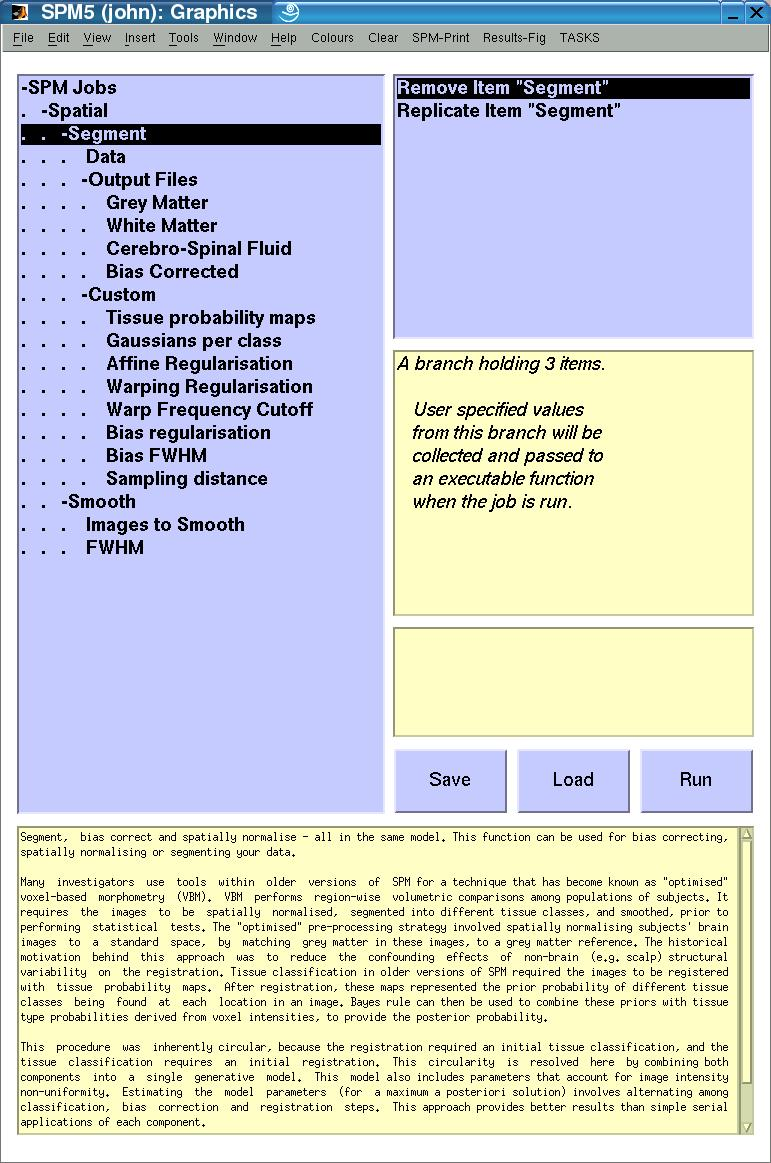
\epsfig{file=ui1,width=70mm} 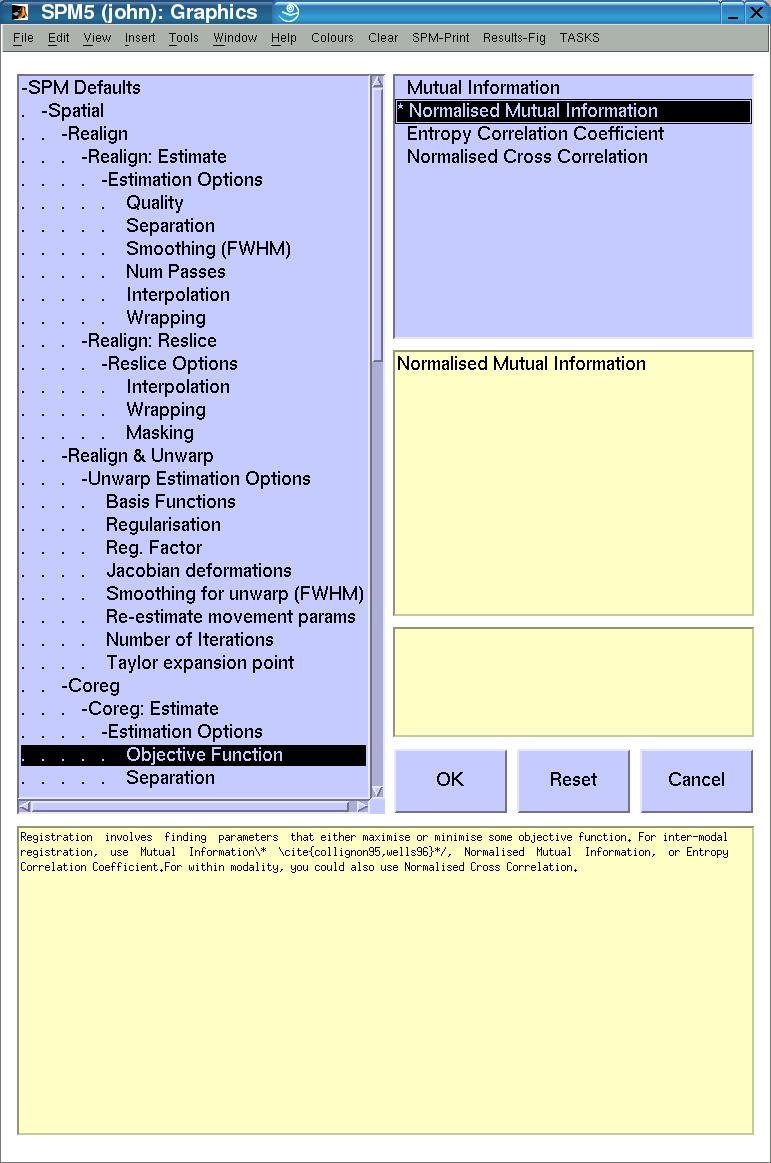
\epsfig{file=ui2,width=70mm} 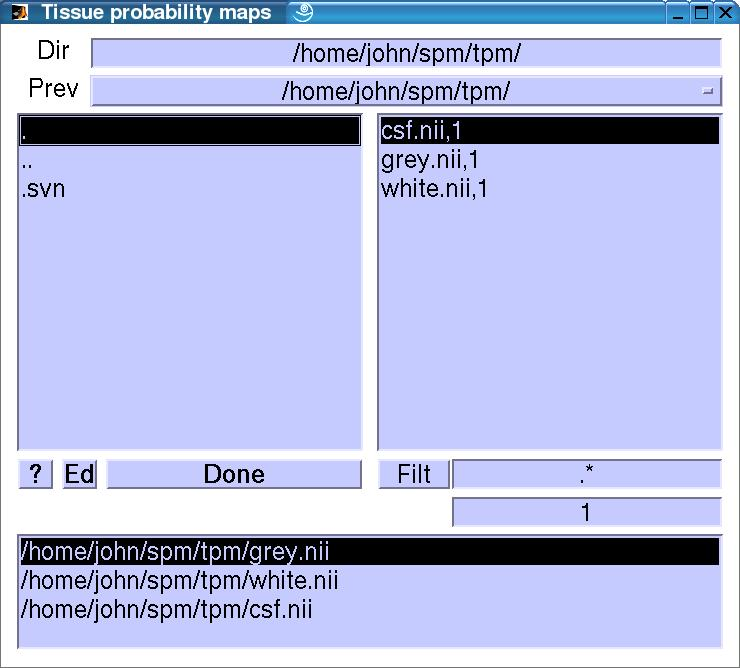
\epsfig{file=ui3,width=70mm} 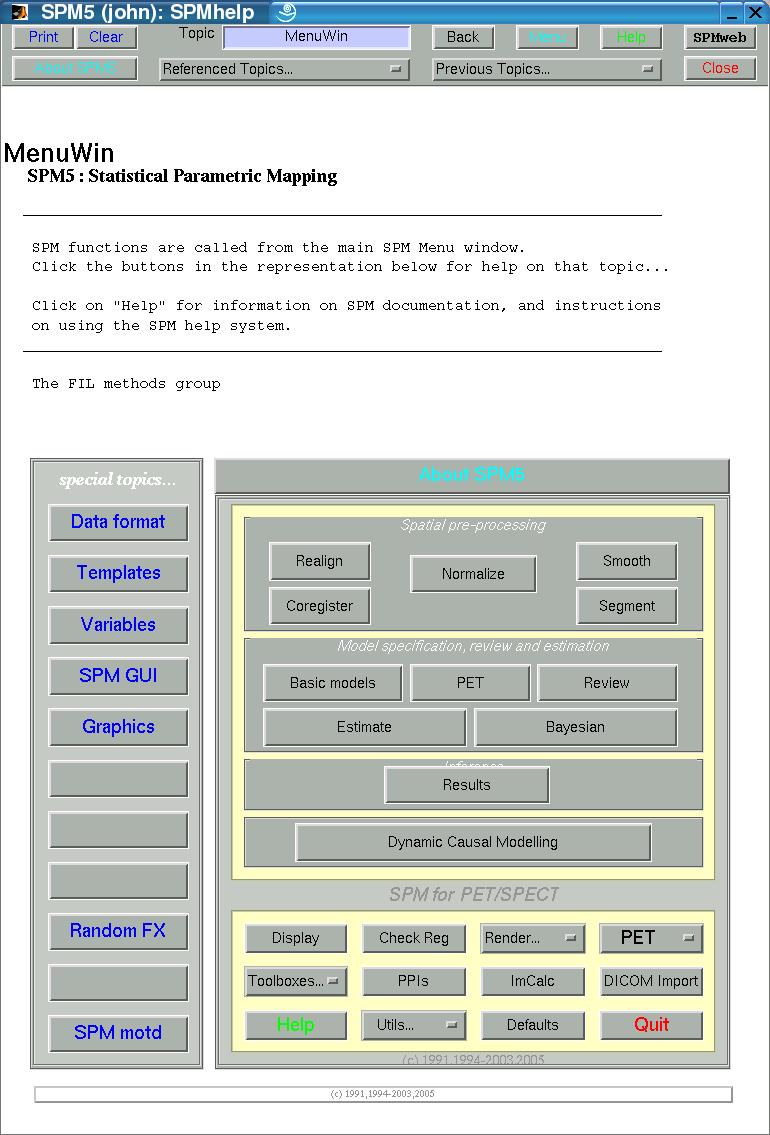
\epsfig{file=ui4,width=70mm}\end{center} \caption{The SPM5 user interface. Top left: The usual user-interface.  Top right: The Defaults user-interface. Bottom left: The file selector (click the (?) button for more information about filtering filenames, or selecting individual volumes within a 4D file. Bottom right: more online help can be obtained via the main help button.} \end{figure} 

\part{Temporal processing}

\include{st}
\include{eeg_filter}
\part{Spatial processing}
\include{realign}
\include{realignunwarp}
\include{coreg}
\include{preproc}
\include{normalise}
\include{smooth}

\part{fMRI Statistics}
\chapter{fMRI model specification}

Statistical analysis of fMRI data uses a mass-univariate approach based on General Linear Models (GLMs). It comprises the following steps (1) specification of the GLM design matrix, fMRI data files and filtering (2) estimation of GLM parameters using classical or Bayesian approaches and (3) interrogation of results using contrast vectors to produce Statistical Parametric Maps (SPMs) or Posterior Probability Maps (PPMs).

The design matrix defines the experimental design and the nature of hypothesis testing to be implemented.  The design matrix has one row for each scan and one column for each effect or explanatory variable. (eg. regressor or stimulus function). You can build design matrices with separable session-specific partitions.  Each partition may be the same (in which case it is only necessary to specify it once) or different. 

Responses can be either event- or epoch related, the only distinction is the duration of the underlying input or stimulus function. Mathematically they are both modeled by convolving a series of delta (stick) or box functions (u), indicating the onset of an event or epoch with a set of basis functions.  These basis functions model the hemodynamic convolution, applied by the brain, to the inputs.  This convolution can be first-order or a generalized convolution modeled to second order (if you specify the Volterra option). The same inputs are used by the Hemodynamic model or Dynamic Causal Models which model the convolution explicitly in terms of hidden state variables. 

Event-related designs may be stochastic or deterministic.  Stochastic designs involve one of a number of trial-types occurring with a specified probability at successive intervals in time.  These probabilities can be fixed (stationary designs) or time-dependent (modulated or non-stationary designs).  The most efficient designs obtain when the probabilities of every trial type are equal. A critical issue in stochastic designs is whether to include null events. If you wish to estimate the evoked response to a specific event type (as opposed to differential responses) then a null event must be included (even if it is not modeled explicitly).

\begin{figure}
\begin{center}
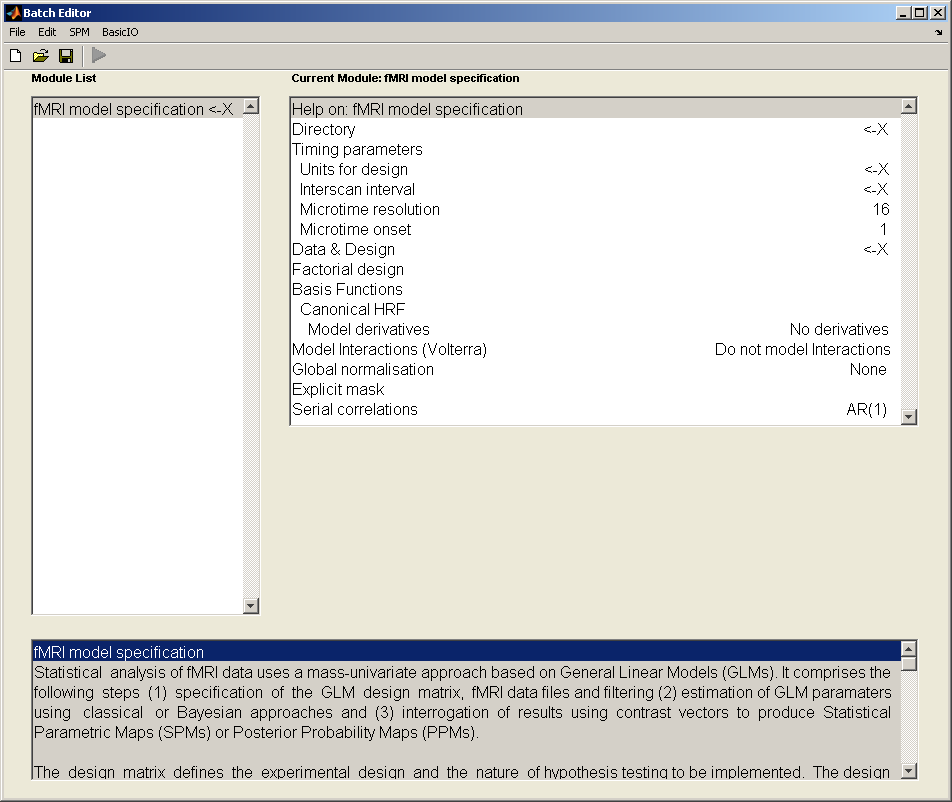
\includegraphics[width=100mm]{fmri_spec/fmri_model}
\end{center}
\caption{\em After starting SPM in fMRI mode, pressing the `Specify 1st-level' button, and then double-clicking on the `+fMRI model specification' text, the SPM graphics window should appear as above. The options under `-fMRI model specification' can be examined by clicking on them. A single click will bring up some help text in the lower subwindow (not shown in the above graphic). A double-click on options prefixed by a '+' will allow you to specify options at a greater level of detail. Options highlighted with a `$<$-X' are mandatory and must be filled in by the user. Each of the options shown above is described in this chapter. \label{spec}}
\end{figure}

In SPM, analysis of data from multiple subjects typically proceeds in two stages using models at two `levels'. The `first level' models are used to implement a within-subject analysis. Typically there will be as many first level models as there are subjects. Analysis proceeds as described using the `Specify first level' and `Estimate' options. The results of these analyses can then be presented as `case studies'. More often, however, one wishes to make inferences about the population from which the subjects were drawn. This is an example of a `Random-Effects (RFX) analysis' (or, more properly, a mixed-effects analysis). In SPM, RFX analysis is implemented using the `summary-statistic' approach where contrast images from each subject are used as summary measures of subject responses. These are then entered as data into a `second level' model. 

Figure~\ref{spec} shows how the SPM graphics window appears during fMRI model specification. 

\section{Timing parameters}

Specify various timing parameters needed to construct the design matrix. This includes the units of the design specification and the interscan interval.

Also, with long TRs you may want to shift the regressors so that they are aligned to a particular slice.  This is effected by changing the microtime resolution and onset. 

\subsection{Units for design}

The onsets of events or blocks can be specified in either scans or seconds.

\subsection{Interscan interval}

Interscan interval, TR, (specified in seconds).  This is the time between acquiring a plane of one volume and the same plane in the next volume.  It is assumed to be constant throughout.

\subsection{Microtime resolution}

In Echo-Planar Imaging (EPI), data is acquired a plane at a time. To acquire a whole volume of data takes at least a second or two.

It is possible, however, that experimental events may occur between scan (volume) acquisition times. This can be specified when building your design matrix either by (i) specifying your design in scans and using non-integer values  or (ii) specifying your design in seconds at a resolution greater than the TR.

SPM takes these timing specifications and builds its regressors using a `microtime' time-scale. The microtime resolution, t, is the number of time-bins per scan. 

Do not change this parameter unless you have a long TR and wish to shift regressors so that they are aligned to a particular slice. 

\subsection{Microtime onset}

The microtime onset, t0, is the first time-bin at which the regressors are resampled to coincide with data acquisition.  If t0 = 1 then the regressors will be appropriate for the first slice.  If you want to temporally realign the regressors so that they match responses in the middle slice then make t0 = t/2 (assuming there is a negligible gap between volume acquisitions).                                           

Do not change the default setting unless you have a long TR. 

A typical use of the t and t0 parameters is to set them to correspond to the results of any slice timing correction you have made eg. if you have 24 slices and have made slice 12 the reference slice you would set t=24, t0=12. 

\section{Data \& Design}

The design matrix defines the experimental design and the nature of hypothesis testing to be implemented.  The design matrix has one row for each scan and one column for each effect or explanatory variable. (e.g. regressor or stimulus function).  Figure~\ref{design} shows an example of a design matrix.

\begin{figure}
\begin{center}
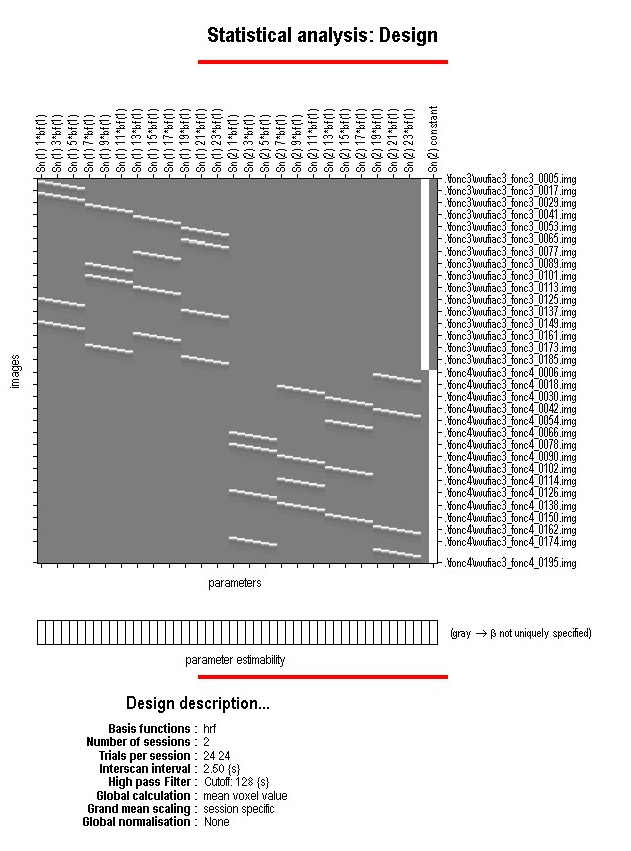
\includegraphics[width=100mm]{fmri_spec/design}
\end{center}
\caption{\em Design matrix for fMRI data from two sessions. There are 24 experimental conditions for each session. The last two columns model the average activity in each session, giving a total of 50 regressors. There are 191 fMRI scans for each session. The overall design matrix therefore has 382 rows and 50 columns. \label{design}}
\end{figure}

You can build design matrices with separable session-specific partitions.  Each partition may be the same (in which case it is only necessary to specify it once) or different.  Responses can be either event- or epoch related, where the latter model involves prolonged and possibly time-varying responses to state-related changes in experimental conditions.  Event-related response are modelled in terms of responses to instantaneous events.  Mathematically they are both modelled by convolving a series of delta (stick) or box-car functions, encoding the input or stimulus function. with a set of hemodynamic basis functions.

\subsection{Subject/Session}

The design matrix for fMRI data consists of one or more separable, session-specific partitions.  These partitions are usually either one per subject, or one per fMRI scanning session for that subject.

\subsubsection{Scans}

Select the fMRI scans for this session.  They must all have the same image dimensions, orientation, voxel size etc. This is implemented using SPM's file selector.

\subsubsection{Conditions}

You are allowed to combine both event- and epoch-related responses in the same model and/or regressor. Any number of condition (event or epoch) types can be specified.  Epoch and event-related responses are modeled in exactly the same way by specifying their onsets [in terms of onset times] and their durations.  Events are specified with a duration of 0.  If you enter a single number for the durations it will be assumed that all trials conform to this duration.For factorial designs, one can later associate these experimental conditions with the appropriate levels of experimental factors. 

\paragraph{Condition}

An array of input functions is constructed, specifying occurrence events or epochs (or both). These are convolved with a basis set at a later stage to give regressors that enter into the design matrix. Interactions of evoked responses with some parameter (time or a specified variate) enter at this stage as additional columns in the design matrix with each trial multiplied by the [expansion of the] trial-specific parameter. The 0th order expansion is simply the main effect in the first column.

\subparagraph{Name}

Condition Name

\subparagraph{Onsets}

Specify a vector of onset times for this condition type. This can be entered using the keyboard eg. typing in `100 300' and then hitting return or `100;300' or `[100,300]' or `[100,300]''.

More usually, however, this specification takes place using variables that have been created before and loaded into matlab. For example, an \verb!my_onsets! cell array\footnote{Cell arrays are usually used in preference to matrices as different event types can then have different numbers of events.} might exist in a file you created earlier called \verb!my_design.mat!. You would then type \verb!load my_design! at the matlab command prompt before pressing the `Specify 1st-level' button. 

You could then specify the onsets for condition 2 by typing in eg. \verb!my_onsets{2}! instead of entering the numbers via the keyboard.


\subparagraph{Durations}

Specify the event durations (in seconds). Epoch and event-related responses are modeled in exactly the same way but by specifying their different durations.  Events are specified with a duration of 0.  If you enter a single number for the durations it will be assumed that all trials conform to this duration. If you have multiple different durations, then the number must match the number of onset times.

\subparagraph{Time Modulation}

This option allows for the characterisation of nonstationary responses.  Specifically, you can model either linear or nonlinear time effects. For example, 1st order modulation would model the stick functions and a linear change of the stick function heights over time. Higher order modulation will introduce further columns that contain the stick functions scaled by time squared, time cubed etc.

\subparagraph{Parametric Modulations}

The stick function itself can be modulated by some parametric variate (this can be time or some trial-specific variate like reaction time) modeling the interaction between the trial and the variate. The events can be modulated by zero or more parameters.

See \cite{parametric_pet,parametric_fmri} for further details of parametric modulations.

\subsubsection{Multiple conditions}

If you have multiple conditions then entering the details a condition at a time is very inefficient. This option can be used to load all the required information in one go. 

You will need to create a \verb!*.mat! file containing the relevant information. This \verb!*.mat! file must include the following cell arrays: names, onsets and durations eg. \verb!names{2}='SSent-DSpeak'!, \verb!onsets{2}=[3 5 19 222]!, \verb!durations{2}=[0 0 0 0]! contain the required details of the second condition. These cell arrays may be made available by your stimulus delivery program eg. COGENT. The duration vectors can contain a single entry if the durations are identical for all events. 

You then need to use SPM's file selector to select this \verb!*.mat! file.

\subsubsection{Regressors}

Regressors are additional columns included in the design matrix, which may model effects that would not be convolved with the haemodynamic response.  One such example would be the estimated movement parameters, which may confound the data.

\paragraph{Regressor}

\subparagraph{Name}

Enter name of regressor eg. First movement parameter

\subparagraph{Value}

Enter the values that the regressor takes. This could also be, for example, the name of a variable in MATLAB's work space that you have previously loaded in from a file. This might be a subjects movement parameters or reaction times.

\subsubsection{Multiple regressors}

If you have mutliple regressors eg. realignment parameters, then entering the details a regressor at a time is very inefficient. This option can be used to load all the required information in one go. 

You will first need to create a *.mat file containing a matrix R. Each column of R will contain a different regressor. When SPM creates the design matrix the regressors will be named R1, R2, R3, ..etc.

You then need to use SPM's file selector to select this \verb!*.mat! file.

\subsubsection{High-pass filter}

The default high-pass filter cutoff is 128 seconds. Slow signal drifts with a period longer than this will be removed. Use `Explore design' to ensure this cut-off is not removing too much experimental variance. This is described later in section~\ref{explore}. High-pass filtering is implemented using a residual forming matrix (i.e. it is not a convolution) and is simply a way to remove confounds without estimating their parameters explicitly.  The constant term is also incorporated into this filter matrix.

\section{Factorial design}

If you have a factorial design then SPM can automatically generate the contrasts necessary to test for the main effects and interactions. 

This includes the F-contrasts necessary to test for these effects at the within-subject level (first level) and the simple contrasts necessary to generate the contrast images for a between-subject (second-level) analysis.

To use this option, create as many factors as you need and provide a name and number of levels for each.  SPM assumes that the condition numbers of the first factor change slowest, the second factor next slowest etc. It is best to write down the contingency table for your design to ensure this condition is met. This table relates the levels of each factor to the conditions. 

For example, if you have 2-by-3 design  your contingency table has two rows and three columns where the the first factor spans the rows, and the second factor the columns. The numbers of the conditions are 1,2,3 for the first row and 4,5,6 for the second. 

See \cite{rnah_anova} for more information on SPM and factorial designs.

\subsection{Factor}

Add a new factor to your experimental design

\subsubsection{Name}

Name of factor, eg. 'Repetition' 

\subsubsection{Levels}

Enter number of levels for this factor, eg. 2

\section{Basis Functions}

SPM uses basis functions to model the hemodynamic response. This could be a single basis function or a set of functions. The most common choice is the `Canonical HRF' with or without time and dispersion derivatives. 

\subsection{Canonical HRF}

Canonical Hemodynamic Response Function (HRF). This is the default option. Contrasts of these effects have a physical interpretation and represent a parsimonious way of characterising event-related responses. This option is also useful if you wish to look separately at activations and deactivations. This is implemented using a t-contrast with a +1 or -1 entry over the canonical regressor. 

\subsubsection{Model derivatives}

Model HRF Derivatives. The canonical HRF combined with time and dispersion derivatives comprise an `informed' basis set, as the shape of the canonical response conforms to the hemodynamic response that is commonly observed. The incorporation of the derivative terms allow for variations in subject-to-subject and voxel-to-voxel responses. The time derivative allows the peak response to vary by plus or minus a second and the dispersion derivative allows the width of the response to vary by a similar amount. 

A positive estimate of the time-derivative regression coefficient implies that the peak hemodynamic response occurs later than usual ie. than would be expected using just the canonical regressor. A positive estimate for the dispersion derivative implies a more dispersed response than usual.

The informed basis set requires an SPM{F} for inference. T-contrasts over just the canonical are perfectly valid but assume constant delay/dispersion. The informed basis set compares favourably with eg. FIR bases on many data sets \cite{rnah_basis}.

\subsection{Other basis sets}

The other basis sets supported by SPM are

\begin{enumerate}
\item{Fourier Set}
\item{Fourier Set (Hanning)}
\item{Gamma Functions}
\item{Finite Impulse Response (FIR)}
\end{enumerate}

For each of these options you must also specify the {\bf window length} which is the length in seconds of the post-stimulus time window that the basis functions span. You must also specify the {\bf order}, that is, how many basis functions to use.

Usually, an informed basis set should be sufficient for most data sets. If this does not provide a good fit to the data it may be worthwhile re-considering how the neuronal events are modelled ie. is the timing correct ? should events be split into subsets ? 

Alternatively, the gamma basis functions are an interesting choice as a particular linear combination of them is actually used to specify the canonical HRF. The FIR approach is of interest as it is equivalent to the method of `selective averaging'. See \cite{rnah_conv} for further details. 

\section{Model Interactions (Volterra)}

Generalized convolution of inputs, $U$, with basis set, $bf$.

For first order expansions the causes are simply convolved (e.g. stick functions) in $U$ by the basis functions in $bf$ to create a design matrix $X$.  For second order expansions new entries appear that correspond to the interaction among the original causes. The basis functions for these effects are two dimensional and are used to assemble the second order kernel. 

Interactions or response modulations can enter at two levels.  Firstly the stick function itself can be modulated by some parametric variate. This can be time or some trial-specific variate like reaction time modeling the interaction between the trial and the variate. Secondly interactions among the trials themselves can be modeled using a Volterra series formulation that accommodates interactions over time (and therefore within and between trial types). 

This last option is useful for accommodating nonlinearities in the hemodynamic response. For example, if two events occur within a second or so of each other then the hemodynamic response to the pair may be less than the sum of the responses to each event when occuring in isolation. This type of `sub-linear' response can be modelled using Volterra kernels. See \cite{balloon} for further details.

\section{Directory}

Select a directory where the SPM.mat file containing the specified design matrix will be written. If this directory already contains an SPM.mat file then SPM will warn you of this before overwriting it, when the specification job is run.

\section{Global normalisation}

SPM can normalise fMRI data in one of two ways. These are selected using the options `None' (the default) and `Scaling'. 

Both methods are based on first estimating the average within-brain fMRI signal, $g_{ns}$, where $n$ denotes scan and $s$ denotes session. If you select `Scaling', SPM will multiply each fMRI value in scan $n$ and session $s$ by $100/g_{ns}$.

If you select `None' then SPM computes the grand mean value, $g_s=\frac{\sum_{n=1}^N g_{ns}}{N}$ where N is the number of scans in that session. This is the fMRI signal averaged over all voxels within the brain and all time points within session $s$. SPM then implements `Session-specific grand mean scaling' by multiplying each fMRI data point in session $s$ by $100/g_s$. 
 
See \cite{ja_global} for further discussion of this issue.

\section{Explicit mask}

Specify an image for explicitly masking the analysis. A sensible option here is to use a segmentation of structural images to specify a within-brain mask. If you select that image as an explicit mask then only those voxels in the brain will be analysed. This both speeds the estimation and restricts SPMs/PPMs to within-brain voxels. Alternatively, if such structural images are unavailable or no masking is required, then leave this field empty.

\section{Serial correlations}

Serial correlations in fMRI time series due to aliased biorhythms and unmodelled neuronal activity can be accounted for using an autoregressive AR(1) model during Classical (ReML) parameter estimation.  

This estimate assumes the same correlation structure for each voxel, within each session.  ReML estimates are then used to correct for non-sphericity during inference by adjusting the statistics and degrees of freedom appropriately.  The discrepancy between estimated and actual correlations are greatest at low frequencies.  Therefore specification of the high-pass filter is particularly important.                                                                                             

Serial correlation can be ignored if you choose the `none' option. Note that the above options only apply if you later specify that your model will be estimated using the Classical (ReML) approach. If you choose Bayesian estimation these options will be ignored. For Bayesian estimation, the choice of noise model (AR model order) is made under the estimation options. See \cite{peb1,vb_fmri_ar} for further discussion of these issues.

\section{Reviewing your design \label{explore}}

After you have completed the SPM `job' file for specifying your fMRI design, and have run it, you will then be able to review your design by pressing the `Review' button in SPM's button window (the top-left window). This is particularly useful, for example, for checking that your experimental variance has not been removed by high-pass filtering, as shown in Figure~\ref{rev4}.

\begin{figure}
\begin{center}
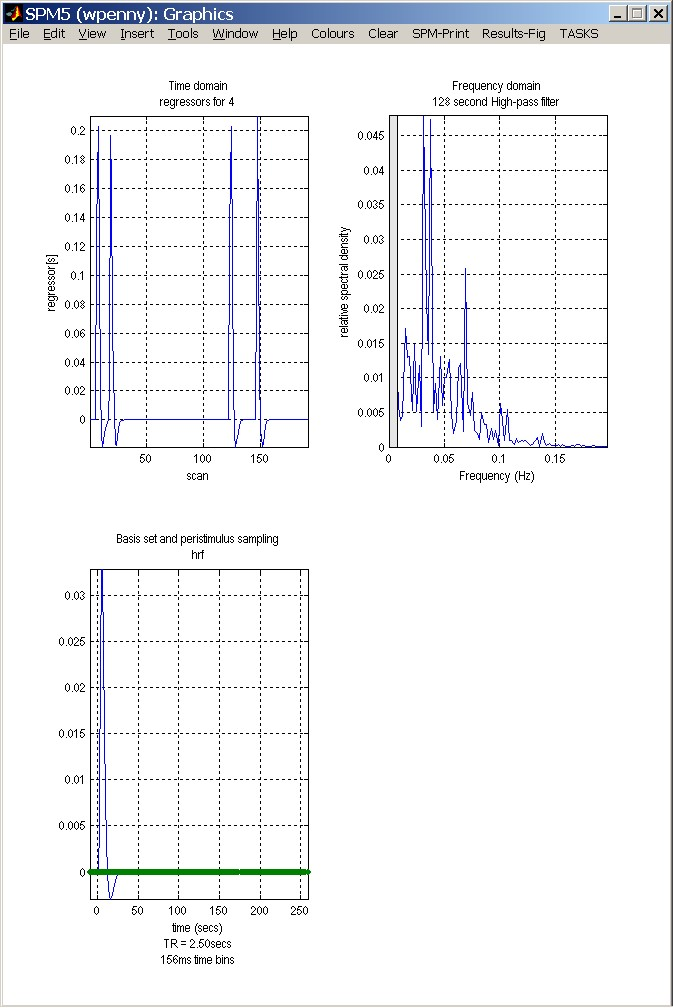
\includegraphics[width=100mm]{fmri_spec/reg4}
\end{center}
\caption{\em After pressing `Review', selecting the pull-down `Design' menu, Explore-$>$Session, and selecting the regressor you wish to look at, you should get a plot similar to the one above. The top row shows time and frequency domain plots of the time-series corresponding to this regressor. In this particular case we have four events. Each event or `stick function' has been convolved with the hemodynamic response function shown in the bottom panel. The frequency domain graph is useful for checking that experimental variance is not removed by high-pass filtering. The grayed out section of the frequency plot shows those frequencies which are removed. For this regressor we have plenty of remaining experimental variance (see the peak at about 0.04Hz). \label{rev4}}
\end{figure}

\chapter{fMRI model estimation \label{Chap:fmri_est}}

Model parameters can be estimated using classical (ReML - Restricted Maximum Likelihood) or Bayesian algorithms. After parameter estimation, the RESULTS button can be used to specify contrasts that will produce Statistical Parametric Maps (SPMs), Effect Size Maps (ESMs) or Posterior Probability Maps (PPMs) and tables of statistics. 

\section{Select SPM.mat}

Select the SPM.mat file that contains the design specification. SPM will output the results of its analysis into this directory. This includes overwriting the SPM.mat file. When the estimation job is run, no warning will be given that the SPM.mat file will be overwritten. A warning is given at the specification stage. When it comes to estimation, SPM assumes that you've now sorted out your directory structures.

\begin{figure}
\begin{center}
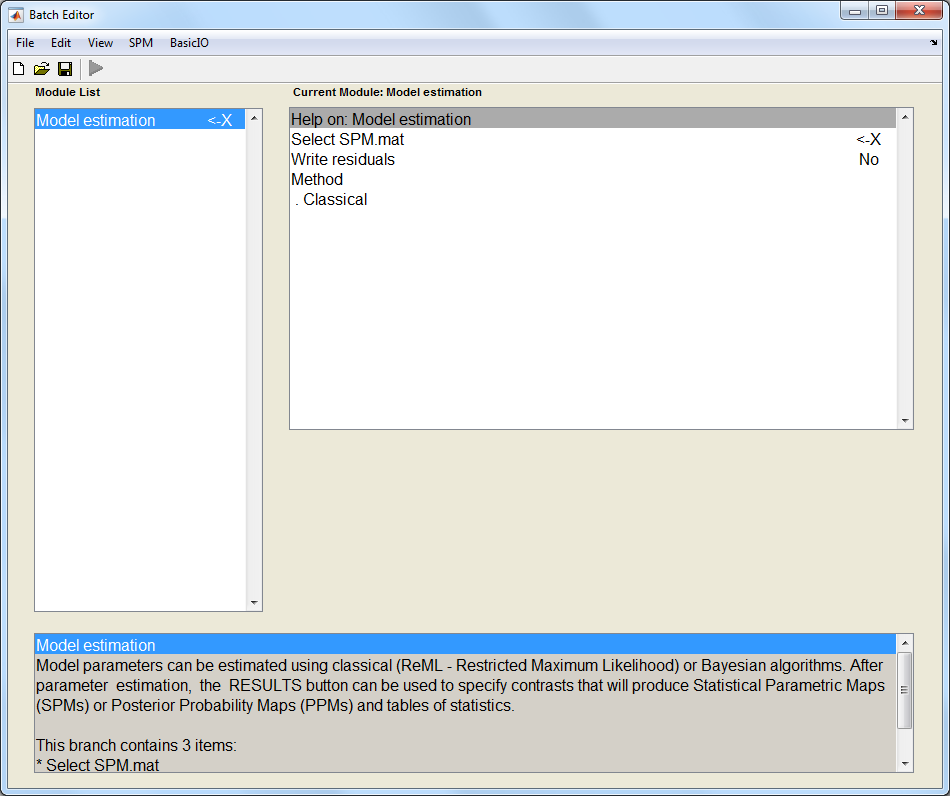
\includegraphics[width=100mm]{fmri_est/est_method}
\end{center}
\caption{\em After starting SPM in fMRI mode, pressing the `Estimate' button, and then double-clicking on the `+fMRI model estimation' text, the SPM graphics window should appear as above. The options under `-fMRI model estimation' can be examined by clicking on them. A single click will bring up some help text in the lower subwindow (not shown in the above graphic). A double-click on options prefixed by a '+' will allow you to specify options at a greater level of detail. Options highlighted with a `$<$-X' are mandatory and must be filled in by the user. Each of the options shown above is described in this chapter. \label{est}}
\end{figure}

\section{Method}

There are three possible estimation procedures for fMRI models (1) classical (ReML) estimation of first or second level models, (2) Bayesian estimation of first level models and (3) Bayesian estimation of second level models. Option (2) uses a Variational Bayes (VB) algorithm that is new to SPM5. Option (3) uses the Empirical Bayes algorithm with global shrinkage priors that was also in SPM2. 

To use option (3) you must have already estimated the model using option (1). That is, for second-level models you must run a ReML estimation before running a Bayesian estimation. This is not necessary for option (2). Bayesian estimation of 1st-level models using VB does not require a prior ReML estimation.

\subsection{Classical}

Model parameters are estimated using Restricted Maximum Likelihood (ReML). This assumes the error correlation structure is the same at each voxel. This correlation can be specified using either an AR(1) or an Independent and Identically Distributed (IID) error model. These options are chosen at the model specification stage. ReML estimation should be applied to spatially smoothed functional images. See \cite{peb1,peb2} for further details of the ReML estimation scheme. After estimation, specific profiles of parameters are tested using a linear compound or contrast with the T or F statistic. The resulting statistical map constitutes an SPM. The SPM{T}/{F} is then characterised in terms of focal or regional differences by assuming that (under the null hypothesis) the components of the SPM (ie. residual fields) behave as smooth stationary Gaussian fields.

The rest of this chapter describes the Bayesian estimation options. So, please skip to the next chapter if you are interested only in classical estimation and inference. 

\subsection{Bayesian 1st-level}

Model parameters are estimated using Variational Bayes (VB). This allows you to specify spatial priors for regression coefficients and regularised voxel-wise AR(P) models for fMRI noise processes. The algorithm does not require functional images to be spatially smoothed. Estimation will take about 5 times longer than with the classical approach. This is why VB is not the default estimation option. The VB approach has been described in a number of papers \cite{vb_fmri_ar,vb2,vb3,will_bayes_srglm}.
                                                          
After estimation, contrasts are used to find regions with effects larger than a user-specified size eg. 1 per cent of the global mean signal. These effects are assessed statistically using a Posterior Probability Map (PPM) \cite{karl_posterior}.

\begin{figure}
\begin{center}
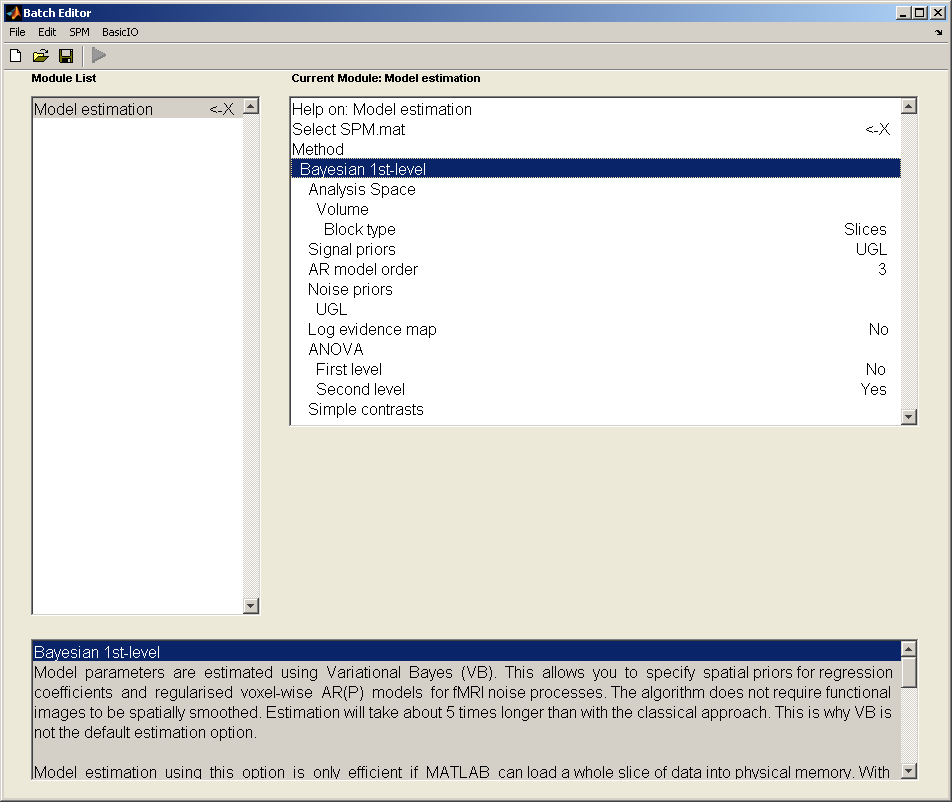
\includegraphics[width=100mm]{fmri_est/bayes_options}
\end{center}
\caption{\em After choosing Bayesian 1st-level under `Method' and then double-clicking on the `+Bayesian 1st-level' text, the SPM graphics window should appear as above. Each of the options shown above is described in this chapter. \label{bayes_options}}
\end{figure}

\subsubsection{Analysis Space}

Because estimation can be time consuming, an option is provided to analyse selected slices rather than the whole volume.

\paragraph{Volume}

You have selected the Volume option. SPM will analyse fMRI time series in all slices of each volume.

\paragraph{Slices}

Enter Slice Numbers. This can be a single slice or multiple slices. If you select a single slice or only a few slices you must be aware of the interpolation options when, after estimation, displaying the estimated images eg. images of contrasts or AR maps. The default interpolation option may need to be changed to nearest neighbour (NN) (see bottom right hand of graphics window) for your slice maps to be visible.

\subsubsection{Signal priors}

\begin{itemize}

\item{[GMRF] Gaussian Markov Random Field. This spatial prior is the recommended option. Regression coefficients at a given voxel are (softly) constrained to be similar to those at nearby voxels. The strength of this constraint is determined by a spatial precision parameter that is estimated from the data. Different regression coefficients have different spatial precisions allowing each putative experimental effect to have its own spatial regularity. }

\item{[LORETA] Low Resolution Tomography Prior. This spatial prior is very similar to the GMRF prior and is a standard choice for MEG/EEG source localisation algorithms. It does, however, have undesirable edge effects.}                                                                                                    

\item{[Global] Global Shrinkage prior. This is not a spatial prior in the sense that regression coefficients are constrained to be similar to neighboring voxels. Instead, the average effect over all voxels (global effect) is assumed to be zero and all regression coefficients are shrunk towards this value in proportion to the prior precision. This is the same prior that is used for Bayesian estimation at the second level (see also \cite{karl_posterior}), except that here the prior precision is estimated separately for each slice. }

\item{[Uninformative] A flat prior. Essentially, no prior information is used. If you select this option then VB reduces to Maximum Likelihood (ML) estimation. This option is useful if, for example, you do not wish to use a spatial prior but wish to take advantage of the voxel-wise AR(P) modelling of noise processes. In this case, you would apply the algorithm to images that have been spatially smoothed. For P=0, ML estimation in turn reduces to Ordinary Least Squares (OLS) estimates, and for P$>$0, ML estimation is equivalent to a weighted least squares (WLS) algorithm but where the weights are different at each voxel. This reflects the different noise correlations at each voxel. }

\end{itemize}

\subsubsection{AR model order}

An AR model order of 3 is the default. Cardiac and respiratory artifacts are periodic in nature and therefore require an AR order of at least 2. In previous work, voxel-wise selection of the optimal model order showed that a value of 3 was the highest order required \cite{vb_fmri_ar}.

Higher model orders have little effect on the estimation time. If you select a model order of zero this corresponds to the assumption that the errors are Independent and Identically Distributed (IID). This AR specification overrides any choices that were made in the model specification stage.

Voxel-wise AR models are fitted separately for each session of data. For each session this therefore produces maps of AR(1), AR(2) etc coefficients in the output directory. 

\subsubsection{Noise priors}

There are three noise prior options.

\begin{itemize}

\item{[GMRF] Gaussian Markov Random Field. This is the default option. This spatial prior is the same as that used for the regression coefficients. Spatial precisions are estimated separately for each AR coefficient eg. the AR(1) coefficient over space, AR(2) over space etc.}

\item{[LORETA] Low Resolution Tomography Prior. See comments on LORETA priors for regression coefficients.}

\item{[Tissue-type] This provides an estimation of AR coefficients at each voxel that are biased towards typical values for that tissue type (eg. gray, white, CSF). If you select this option you will need to then select files that contain tissue type maps (see below). These are typically chosen to be Grey Matter, White Matter and CSF images derived from segmentation of registered structural scans.}

\end{itemize}
                                                                                                            
Previous work has shown that there is significant variation in AR values with tissue type. However, GMRF priors have previously been favoured by Bayesian model comparison \cite{will_bayes_srglm}.

\subsubsection{ANOVA}

Perform 1st or 2nd level Analysis of Variance.

\paragraph{First level}

This is implemented using Bayesian model comparison as described in \cite{will_bayes_srglm}. For example, to test for the main effect of a factor two models are compared, one where the levels are represented using different regressors and one using the same regressor. This therefore requires explicit fitting of several models at each voxel and is computationally demanding (requiring several hours of computation). The recommended option is therefore NO.

To use this option you must have already specified your factorial design during the model specification stage. 

\paragraph{Second level}

This option tells SPM to automatically generate the simple contrasts that are necessary to produce the contrast images for a second-level (between-subject) ANOVA. Naturally, these contrasts can also be used to characterise simple effects for each subject. 

With the Bayesian estimation option it is recommended that contrasts are computed during the parameter estimation stage (see 'simple contrasts' below). The recommended option here is therefore YES.

To use this option you must have already specified your factorial design during the model specification stage. 

If you wish to use these contrast images for a second-level analysis then you will need to spatially smooth them to take into account between-subject differences in functional anatomy ie. the fact that one persons V5 may be in a different position than anothers. 

\subsubsection{Simple contrasts}

`Simple' contrasts refers to a contrast that spans one-dimension ie. to assess an effect that is increasing or decreasing.

If you have a factorial design then the contrasts needed to generate the contrast images for a 2nd-level ANOVA (or to assess these simple effects within-subject) can be specified automatically using the ANOVA-$>$Second level option.

When using the Bayesian estimation option it is computationally more efficient to compute the contrasts when the parameters are estimated. This is because estimated parameter vectors have potentially different posterior covariance matrices at different voxels and these matrices are not stored. If you compute contrasts post-hoc these matrices must be recomputed. This uses an approximate reconstruction based on a Taylor series expansion described in \cite{vb3}. It is therefore recommended to specify as many contrasts as possible prior to parameter estimation.

If you wish to use these contrast images for a second-level analysis then you will need to spatially smooth them to take into account between-subject differences in functional anatomy ie. the fact that one persons V5 may be in a different position than anothers. 

\paragraph{Simple contrast}

\subparagraph{Name}

Name of contrast eg. `Positive Effect'

\subparagraph{Contrast vector}

These contrasts are used to generate PPMs which characterise effect sizes at each voxel. This is different to SPMs in which eg. maps of t-statistics show the ratio of the effect size to effect variability (standard deviation). SPMs are therefore a-dimensional. This is not the case for PPMs as the size of the effect is of primary interest. Some care is therefore needed about the scaling of contrast vectors. For example, if you are interested in the differential effect size averaged over conditions then the contrast $[0.5, 0.5, -0.5, -0.5]$ would be more suitable than the $[1, 1, -1, -1]$ contrast which looks at the differential effect size summed over conditions. 

\subsection{Bayesian 2nd-level}

Bayesian estimation of 2nd level models. This option uses the Empirical Bayes algorithm with global shrinkage priors that was previously implemented in SPM2. It is described in detail in \cite{karl_posterior}.

Use of the global shrinkage prior embodies a prior belief that, on average over all voxels, there is no net experimental effect. Some voxels will respond negatively and some positively with a variability determined by the prior precision. This prior precision can be estimated from the data using Empirical Bayes. 

\section{Output files}

After estimation a number of files are written to the output directory. These are

\begin{itemize}
\item{An \verb!SPM.mat! file containing specification of the design and estimated model parameters}
\end{itemize}

\subsection{Classical 1st-level}

For classical 1st-level models the following files are also produced

\begin{itemize}

\item{Images of estimated regression coefficients  \verb!beta_000k.img! where $k$ indexes the $k$th regression coefficient.}

\item{An image of the variance of the error \verb!ResMS.img!.}

\item{An image \verb!mask.img! indicating which voxels were included in the analysis.}

\item{The image \verb!RPV.img!, the estimated resels per voxel.}

\item{If contrasts have been specified SPM also writes \verb!con_000i.img!  if the $i$th contrast is a t-contrast and the extra sum of squares image \verb!ess_000i.img! if it is an F-contrast.} 

\end{itemize}

Type \verb!help spm_spm! at the matlab command prompt for further information.

\subsection{Bayesian 1st-level}

For Bayesian 1st-level models the following files are also produced

\begin{itemize}

\item{Images of estimated regression coefficients  \verb!Cbeta_000k.img! where $k$ indexes the $k$th regression coefficient. These filenames are prefixed with a `C' indicating that these are the mean values of the `Conditional' or `Posterior' density.}

\item{Images of error bars/standard deviations on the regression coefficients \verb!SDbeta_000k.img!.}

\item{An image of the standard deviation of the error \verb!Sess1_SDerror.img!.}

\item{An image \verb!mask.img! indicating which voxels were included in the analysis.}

\item{If a non-zero AR model order is specified then SPM also writes images \verb!Sess1_AR_000p.img! where $p$ indexes the $p$th AR coefficient.}

\item{If contrasts have been specified SPM also writes \verb!con_000i.img! and \verb!con_sd_000i.img! which are the mean and standard deviation of the $i$th pre-defined contrast.} 

\end{itemize}

Each of these images can be inspected using the `Display' button. Type \verb!help spm_spm_vb! at the matlab command prompt for further information.

\section{Model comparison}

Once you have estimated a model you can use SPM's results button to look at the results. You can also extract fMRI data from regions of interest using the ROI button. You can then compare GLMs based on different hemodynamic basis sets using the Bayesian model evidence. 

This is described in \cite{will_bayes_srglm} and implemented using the command line option `spm\_vb\_roi\_basis'. This requires a VOI filename (created using the ROI button) and an SPM data structure. Type `help spm\_vb\_roi\_basis' at the matlab command prompt for further information. Figure~\ref{basis} shows an example output from the function indicating that, for the data in this brain region, an informed basis set has the highest model evidence.

\begin{figure}
\begin{center}
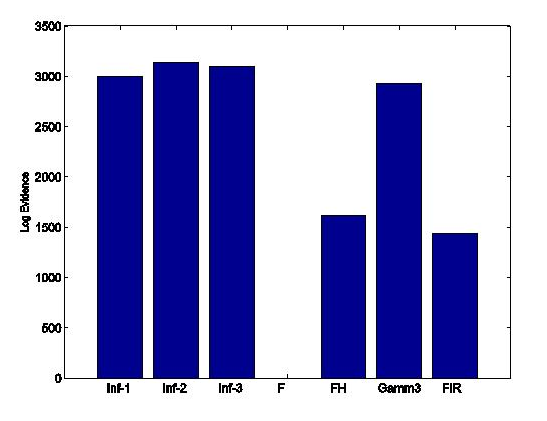
\includegraphics[width=150mm]{fmri_est/basis}
\end{center}
\caption{\em This plot shows the model evidence for a number of different hemodynamic basis sets: Inf1 - Canonical HRF, Inf2 - Canonical plus temporal derivative, Inf3 - Canonical plus temporal and dispersion derivatives, F - Fourier, FH - Fourier with a Hanning Window, Gamm3 - 3 Gamma basis functions and FIR - a Finite Impulse Response function. An informed basis set provides the best model of the data for the selected region.  \label{basis}}
\end{figure}


\part{Utilities}
\include{disp}
\include{checkreg}
\include{imcalc}
\include{dicom}
\include{minc}
\include{ecat}
\include{runbatch}
\include{cdir}
\include{md}
\include{defs}
\include{ui}

\part{Data sets}
\chapter{Auditory fMRI data \label{Chap:data:auditory}}
 
This data set comprises whole brain BOLD/EPI images acquired on a modified 2T Siemens MAGNETOM Vision system. Each acquisition consisted of 64 contiguous slices (64$\times$64$\times$64 3$\times$3mm$\times$3 mm$^3$ voxels). Acquisition took 6.05s, with the scan to scan repeat time (TR) set arbitrarily to 7s.

96 acquisitions were made (TR=7s) from a single subject, in blocks of 6, giving 16 42s blocks. The condition for successive blocks alternated between rest and auditory stimulation, starting with rest. Auditory stimulation was bi-syllabic words presented binaurally at a rate of 60 per minute. The functional data starts at acquisition 4, image \texttt{fM00223\_004}. Due to T1 effects it is advisable to discard the first few scans (there were no ``dummy'' lead-in scans). A structural image was also acquired: \texttt{sM00223\_002}. These images are stored in Analyze format and are available from the SPM site \footnote{Auditory fMRI data: \url{http://www.fil.ion.ucl.ac.uk/spm/data/}}. This data set was the first ever collected and analysed in the Functional Imaging Laboratory (FIL) and is known locally as the mother of all experiments (MoAE).

To analyse the data, first create a new directory \texttt{DIR},  eg. \texttt{c:$\backslash$data$\backslash$auditory}, in which to place the results of your analysis. Then create 3 subdirectories (i) \texttt{jobs}, (ii) \texttt{classical} and (iii) \texttt{bayesian}. As the analysis proceeds these directories will be filled with job-specification files, design matrices and models estimated using classical or Bayesian methods.

Start up \matlab\, enter your jobs directory and type \texttt{spm fmri} at the \matlab\ prompt. SPM will then open in fMRI mode with three windows (1) the top-left or ``Menu'' window, (2) the bottom-left or ``Interactive'' window and (3) the right-hand or ``Graphic'' window. Analysis then takes place in three major stages (i) spatial pre-processing, (ii) model specification, review and estimation and (iii) inference. These stages organise the buttons in SPM's base window.

\begin{figure}
\begin{center}
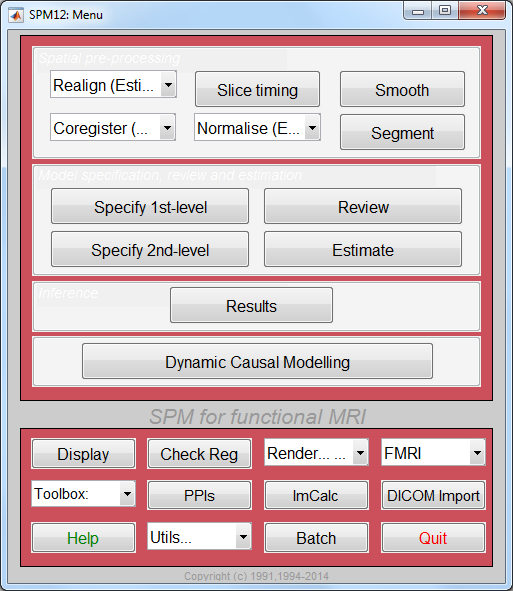
\includegraphics[width=100mm]{auditory/command}
\caption{\em The SPM base window comprises three sections i) spatial pre-processing, (ii) model specification, review and estimation and (iii) inference. \label{aud_command}}
\end{center}
\end{figure}

\section{Spatial pre-processing}

\subsection{Realignment}

Under the spatial pre-processing section of the SPM base window select textsc{Realign (Est \& Res)} from the \textsc{Realign} pulldown menu. This will call up a realignment job specification in the batch editor. Then
\begin{itemize}
\item Highlight data, select ``New Session'', then highlight the newly created ``Session'' option.
\item Select ''Specify Files'' and use the SPM file selector to choose all of your functional images eg. ``\texttt{fM000*.img}''. There should be 96 files.
\item Save the job file as eg. \texttt{DIR$\backslash$jobs$\backslash$realign.mat}.
\item Press the \texttt{RUN} button in the batch editor (green arrow).
\end{itemize}

This will run the realign job which will write realigned images into the directory where the functional images are. These new images will be prefixed with the letter ``\texttt{r}''. SPM will then plot the estimated time series of translations and rotations shown in Figure~\ref{aud_realign}. These data are also saved to a file eg. \texttt{rp\_fM00223\_004.txt}, so that these variables can be used as regressors when fitting GLMs. This allows movements effects to be discounted when looking for brain activations.

SPM will also create a mean image eg. \texttt{meanfM00223\_004.img} which will be used in the next step of spatial processing - coregistration.

\begin{figure}
\begin{center}
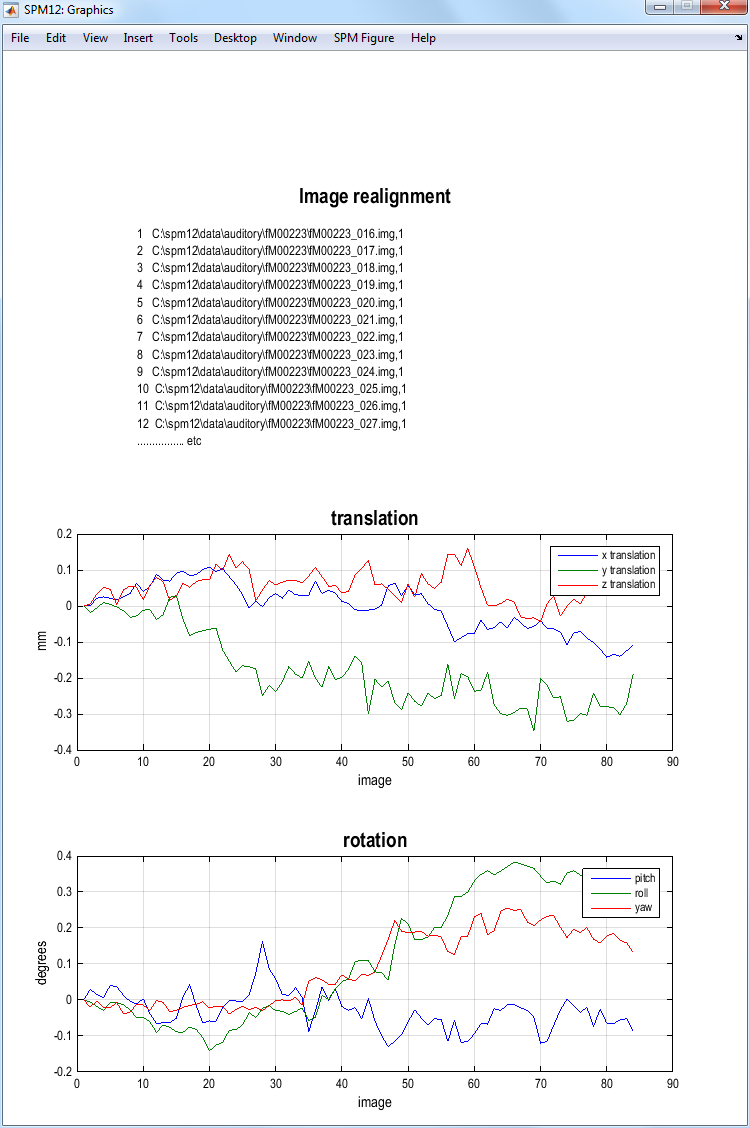
\includegraphics[width=100mm]{auditory/realign}
\caption{\em Realignment of Auditory data.\label{aud_realign}}
\end{center}
\end{figure}

\subsection{Coregistration}

Select \textsc{Coregister (Estimate)} from the \textsc{Coregister} pulldown. This will call up the specification of a coregistration job in the batch editor. 

\begin{itemize}
\item Highlight ``Reference Image'' and then select the mean fMRI scan from realignment eg. \texttt{meanfM00223\_004.img}.
\item Highlight ``Source Image'' and then select the structural image eg. \texttt{sM00223\_002.img}.
\item Press the Save button and save the job as \texttt{coreg.job}.
\item Then press the \texttt{RUN} button.
\end{itemize}

SPM will then implement a coregistration between the structural and functional data that maximises the mutual information. The image in figure~\ref{aud_coreg} should then appear in the graphics window. SPM will have changed the header of the source file which in this case is the structural image \texttt{sM00223\_002.hdr}.
\begin{figure}
\begin{center}
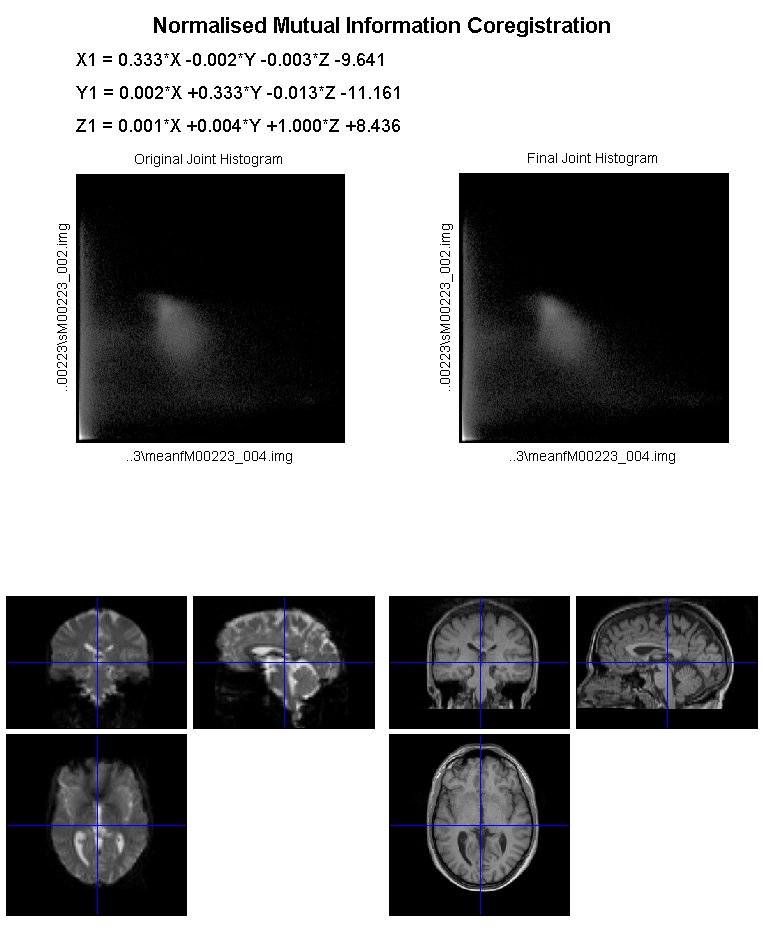
\includegraphics[width=100mm]{auditory/coreg}
\caption{\em Mutual Information Coregistration of Auditory data.\label{aud_coreg}}
\end{center}
\end{figure}

The \textsc{Check Reg} facility is useful here, to check the results of coregistration. Press the \textsc{Check Reg} button in the lower section of the base window and then the select the ``Reference'' and ``Source'' Images specified above ie \texttt{meanfM00223\_004.img} and \texttt{sM00223\_002.img}. SPM will then produce an image like that shown in Figure~\ref{aud_checkreg} in the Graphics window. You can then use your mouse to navigate these images to confirm that there is an anatomical correspondence.

\begin{figure}
\begin{center}
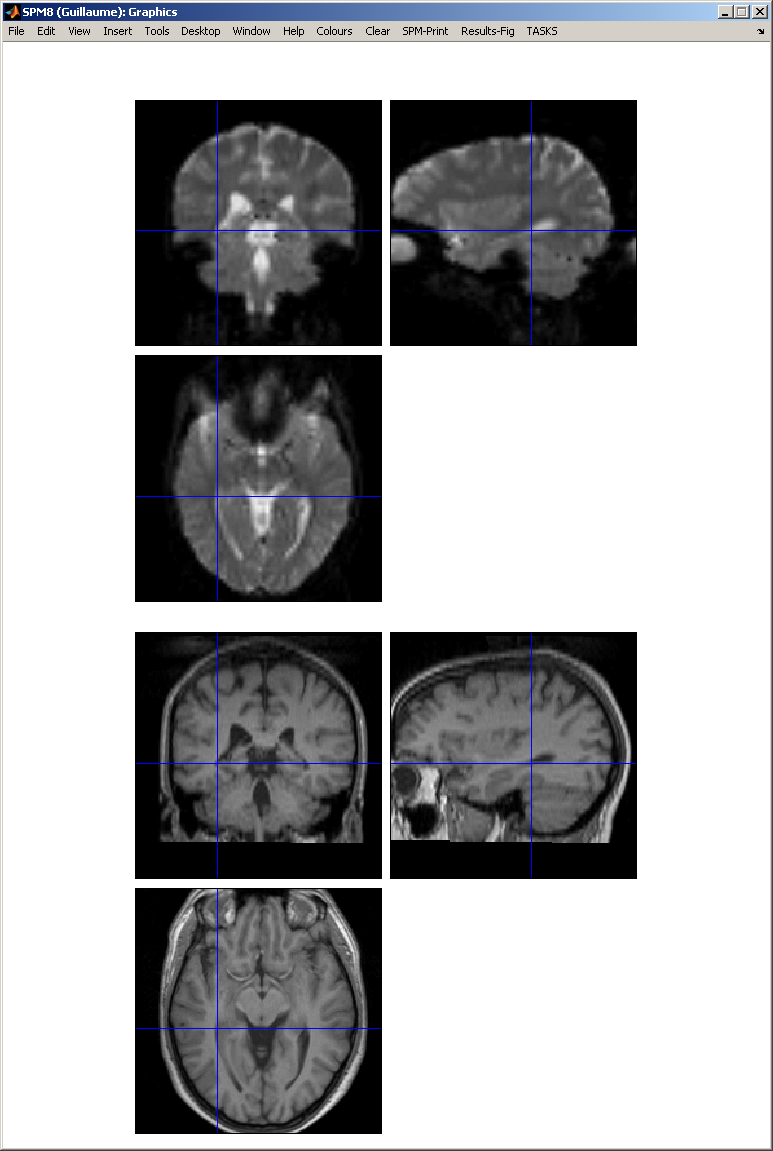
\includegraphics[width=100mm]{auditory/checkreg}
\caption{\em Checking registration of functional and ``registered'' structural data. \label{aud_checkreg}}
\end{center}
\end{figure}

\subsection{Segmentation}

Press the \textsc{Segment} button. This will call up the specification of a segmentation job in the batch editor. Highlight the Data field and then select the subjects registered anatomical image eg. \texttt{sM00223\_002.img}. Save the job file as \texttt{segment.mat} and then press \texttt{RUN}. SPM will segment the structural image using the default tissue probability maps as priors. 

Faster, though perhaps less optimal results can be obtained by eg. reducing the number of Gaussians per class from [2 2 2 4] to eg. [1 1 1 4], increasing the sampling distance from eg. 3 to 4mm. These options can be edited under the ``Custom'' sub-menu and saved before the job is run. The results obtained in figure~\ref{aud_gray} were obtained using the default values.

SPM will create, by default, gray and white matter images and bias-field corrected structural image. These can be viewed using the CheckReg facility as described in the previous section. Figure~\ref{aud_gray} shows the gray matter image, \texttt{c1sM0023\_002.img} along with the original structural. Figure~\ref{aud_bias} shows the structural and bias-corrected image, \texttt{msM0023\_002.img}.

\begin{figure}
\begin{center}
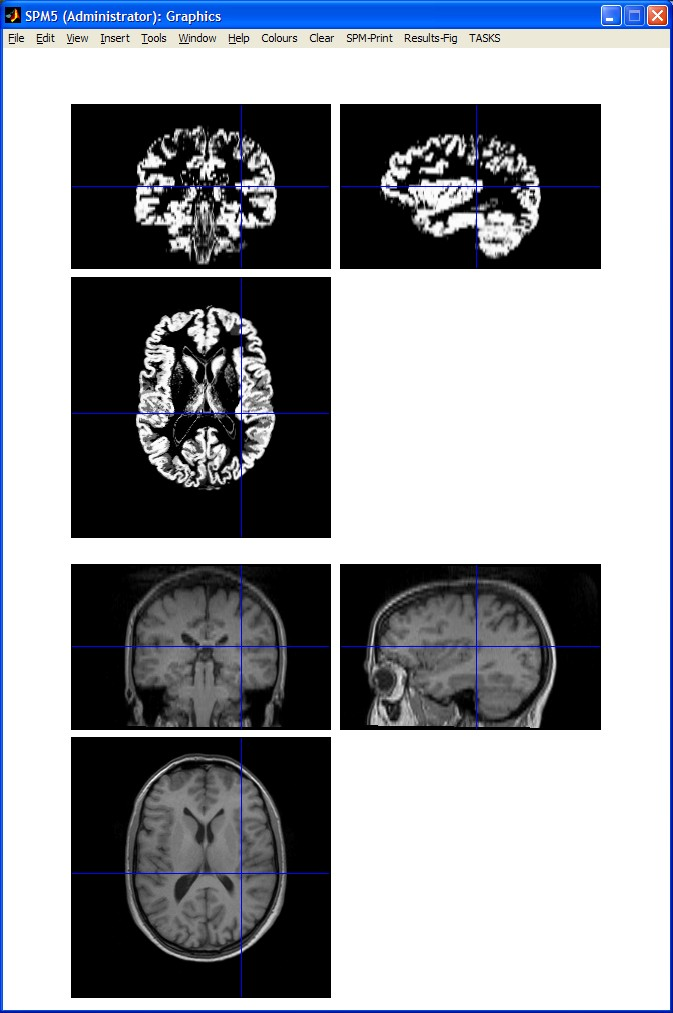
\includegraphics[width=100mm]{auditory/gray}
\caption{\em Gray matter image and ``registered'' structural image.\label{aud_gray}}
\end{center}
\end{figure}

\begin{figure}
\begin{center}
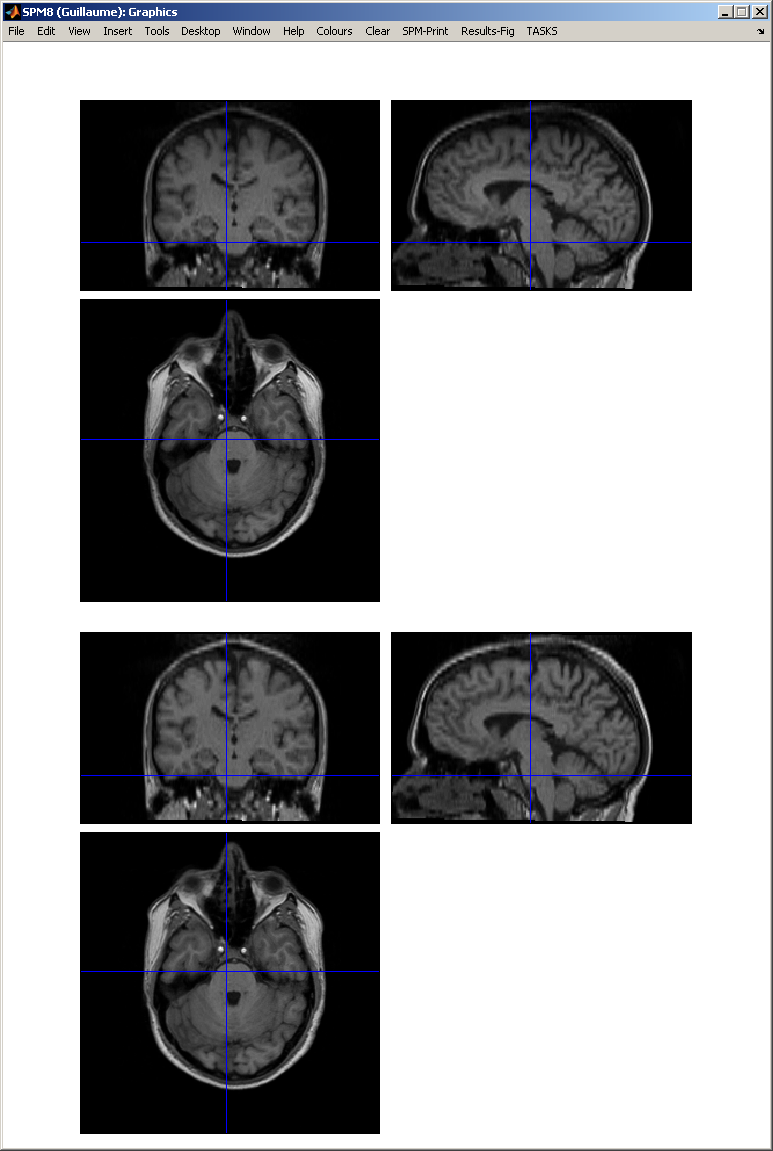
\includegraphics[width=100mm]{auditory/bias}
\caption{\em Structural image (top) and bias-corrected structural image (bottom). Notice that the original structural is darker at the top than at the bottom. This non-uniformity has been removed in the bias-corrected image.\label{aud_bias}}
\end{center}
\end{figure}

SPM will also write a spatial normalisation eg. \texttt{sM00223\_0020\_seg\_sn.mat} and inverse spatial normalisation parameters \texttt{sM00223\_0020\_seg\_inv\_sn.mat} to files in the original structural directory. These can be used to normalise the functional data. 

\subsection{Normalise}

Select \textsc{Normalise (Write)} from the \textsc{Normalise} pulldown menu. This will call up the specification of a normalise job in the batch editor. 

\begin{itemize}
\item Highlight ``Data'', select New ``Subject'',
\item Highlight ``Parameter File'' and select the \texttt{sM00223\_0020\_seg\_sn.mat} file that you created in the previous section,
\item Highlight images to write and select all of the realigned functional images \texttt{rfM000*.img}. Note: This can be done efficiently by changing the filter in the SPM file selector to \texttt{\^r.*}. SPM will then only list those files beginning with the letter \texttt{r} ie. those that have been realigned. You can then right click over the listed files, choose ``Select all'' and press ``Done''.
\item Open ``Writing Options'', and change ``Voxel sizes'' from [2 2 2] to [3 3 3].\footnote{This step is not strictly necessary. It will write images out at a resolution closer to that at which they were acquired. This will speed up subsequent analysis and is necessary, for example, to make Bayesian fMRI analysis computationally efficient.}
\item Press ``Save'', save the job as \texttt{normalise.mat} and then press the \texttt{RUN} button.
\end{itemize}

SPM will then write spatially normalised files to the functional data directory. These files have the prefix \texttt{w}.

If you wish to superimpose a subject's functional activations on their own anatomy\footnote{Beginners may wish to skip this step, and instead just superimpose functional activations on an ``average structural image''.} you will also need to apply the spatial normalisation parameters to their (bias-corrected) anatomical image. To do this

\begin{itemize}
\item Select \textsc{Normalise (Write)}, highlight ``Data'', select ``New Subject''.
\item Highlight ``Parameter File'', select the  \texttt{sM00223\_0020\_seg\_sn.mat} file that you created in the previous section, press ``Done''.
\item Highlight ``Images to Write'', select the bias-corrected structural eg. \texttt{msM00223\_002.img}, press ``Done''.
\item Open ``Writing Options'', select voxel sizes and change the default [2 2 2] to [1 1 3] which corresponds to the original resolution of the images.
\item Save the job as \texttt{norm\_struct.mat} and press the \texttt{Run} button.
\end{itemize}

\subsection{Smoothing}

Press the \textsc{Smooth} button\footnote{The smoothing step is unnecessary if you are only interested in Bayesian analysis of your functional data.}. This will call up the specification of a smooth job in the batch editor.

\begin{itemize}
\item Select ``Images to Smooth'' and then select the spatially normalised files created in the last section eg. \texttt{\^wrf.*}.
\item Highlight ``FWHM'' and change [8 8 8] to [6 6 6]. This will smooth the data by 6mm in each direction.
\item Save the job as \texttt{smooth.mat} and press the \texttt{Run} button.
\end{itemize}

An example of functional image and its smoothed version is displayed on Figure~\ref{aud_smooth}.

\begin{figure}
\begin{center}
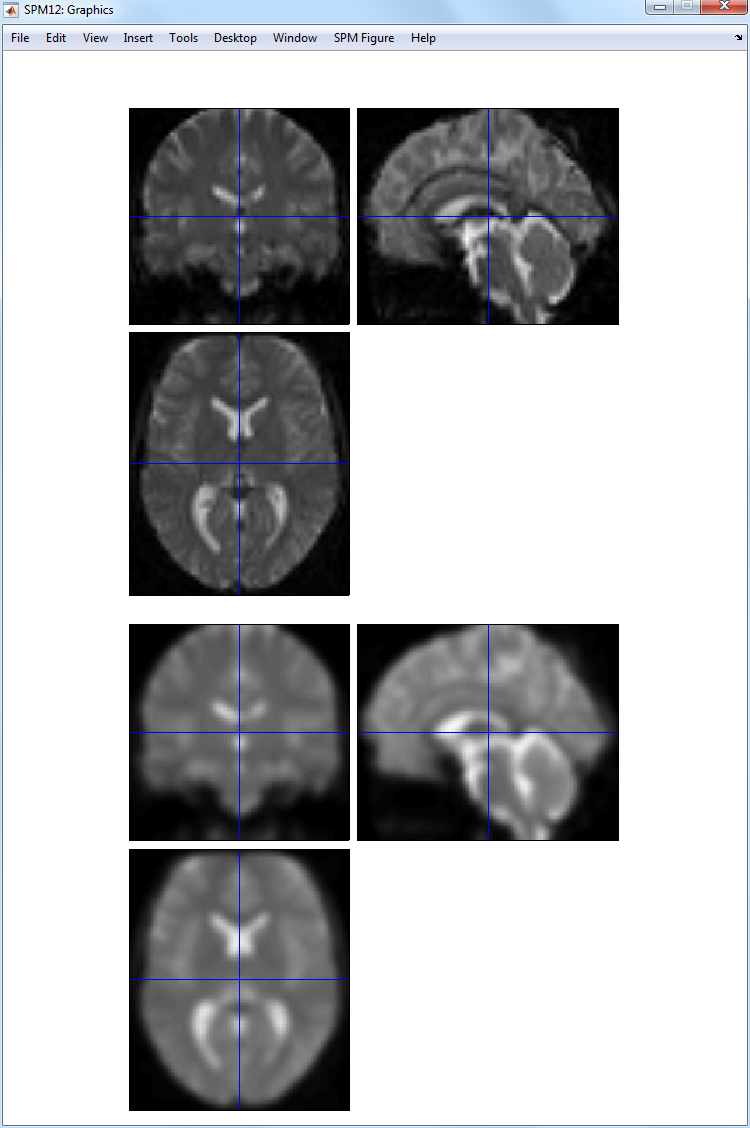
\includegraphics[width=100mm]{auditory/smooth}
\caption{\em Functional image (top) and 6mm-smoothed functional image (bottom). These images were obtained using SPM's ``CheckReg'' facility. \label{aud_smooth}}
\end{center}
\end{figure}

\section{Model specification, review and estimation}

To avoid T1 effects in the initial scans of an fMRI time series we recommend discarding the first few scans. To make this example simple, we'll discard the first complete cycle (12 scans, 04-15), leaving 84 scans, image files 16-99. This is best done by moving these files to a different directory.

Press the ``Specify 1st-level'' button. This will call up the specification of an fMRI specification job in the batch editor. Then

\begin{itemize}
\item Open the ``Timing parameters'' option.
\item Highlight ``Units for design'' and select ``Scans''.
\item Highlight ``Interscan interval'' and enter 7.
\item Highlight ``Data and Design'' and select ``New Subject/Session''. Then open the newly created ``Subject/Session'' option.
\item Highlight ``Scans'' and use SPM's file selector to choose the 84 smoothed, normalised functional images ie  \texttt{swrfM00223\_016.img} to \texttt{swrfM00223\_099.img}. These can be selected easily using the \texttt{\^s.*'} filter, and select all (provided you have moved the scans 4 to 15 into a different directory). Then press ``Done''.
\item Highlight ``Condition'' and select ``New condition''.
\item Open the newly created ``Condition'' option. Highlight ``Name'' and enter ``active''. Highlight ``Onsets'' and enter ``6:12:84''. Highlight ``Durations'' and enter ``6''.
\item Highlight ``Directory'' and select the \texttt{DIR/classical} directory you created earlier.
\item Save the job as \texttt{specify.mat} and press the \texttt{Run} button.
\end{itemize}

SPM will then write an \texttt{SPM.mat} file to the \texttt{DIR/classical} directory. It will also plot the design matrix, as shown in Figure~\ref{aud_design}. 

\begin{figure}
\begin{center}
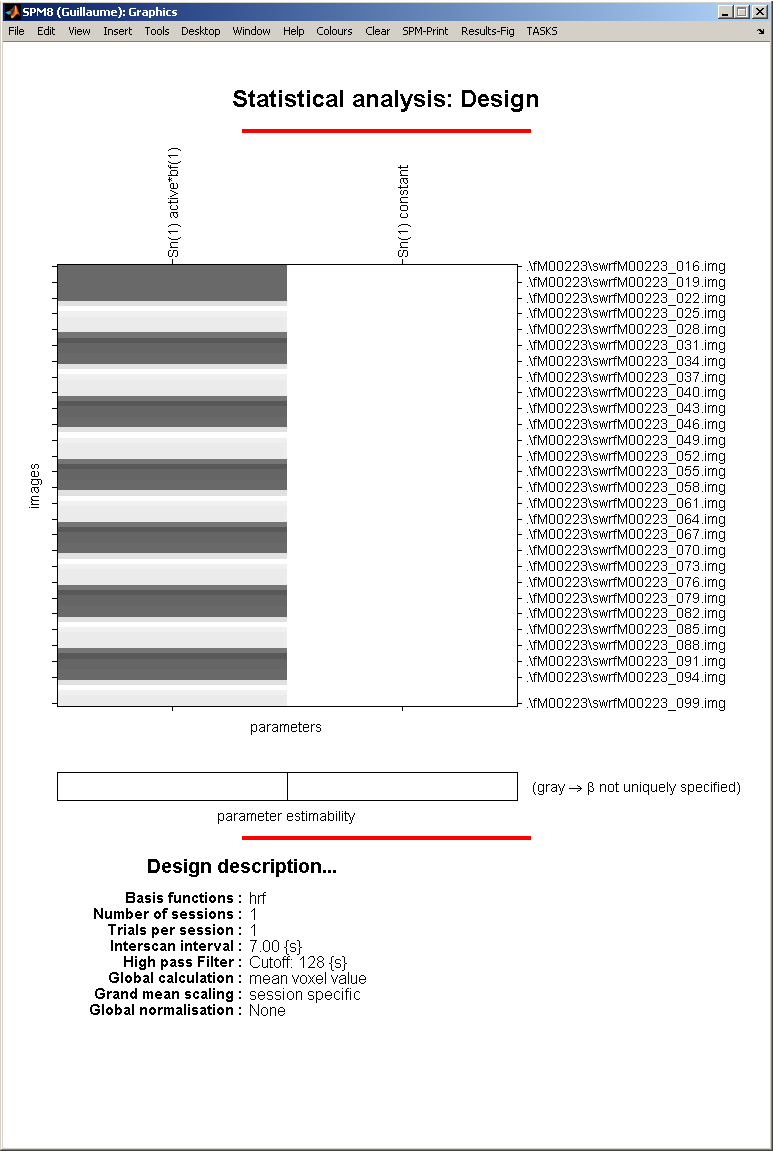
\includegraphics[width=80mm]{auditory/design}
\caption{\emph{\texttt{Design matrix}: The filenames on the right-hand side of the design matrix indicate the scan associated with each row.\label{aud_design}}}
\end{center}
\end{figure}

At this stage it is advisable to check your model specification using SPM's review facility which is accessed via the ``Review'' button. This brings up a ``design'' tab on the interactive window clicking on which produces a pulldown menu. If you select the first item ``Design Matrix'' SPM will produce the image shown in Figure~\ref{aud_design}. If you select ``Explore'' then ``Session 1'' then ``active'', SPM will produce the plots shown in Figure~\ref{aud_explore}.

\begin{figure}
\begin{center}
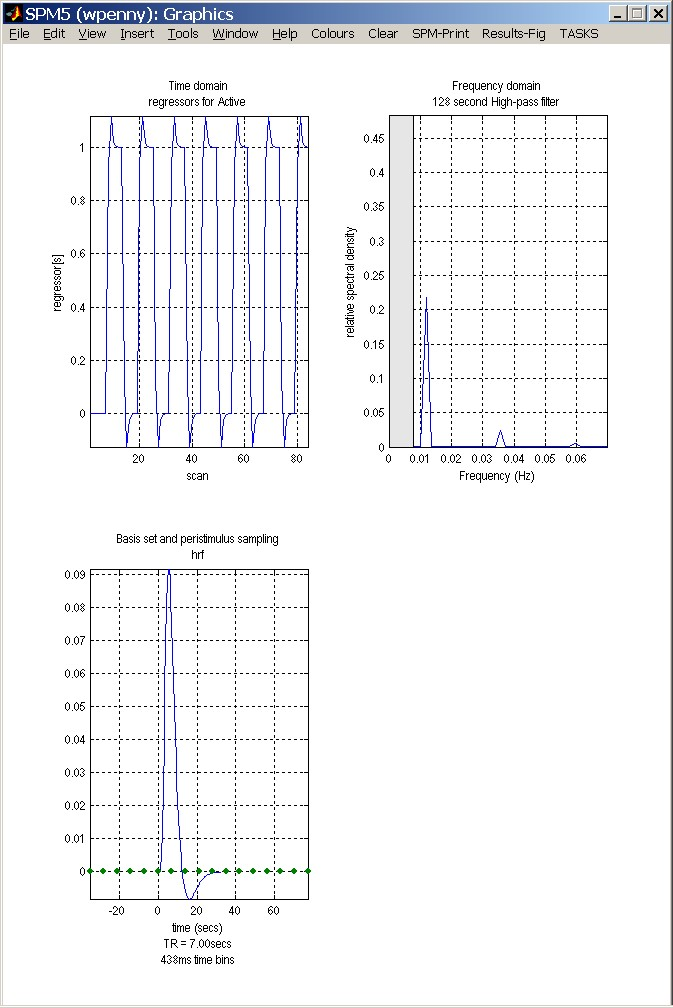
\includegraphics[width=80mm]{auditory/explore}
\caption{\emph{\texttt{Exploring the design matrix in Figure~\ref{aud_design}}: This shows the time series of the ``active'' regressor (top left), a frequency domain plot of the active regressor (top right) and the basis function used to convert assumed neuronal activity into hemodynamic activity. In this model we used the default option - the canonical basis function. The frequency domain plot shows that the frequency content of the ``active'' regressor is above the set frequencies that are removed by the High Pass Filter (HPF) (these are shown in gray - in this model we accepted the default HPF cut-off of 128s or 0.008Hz). \label{aud_explore}}}
\end{center}
\end{figure}

If you select the second item on the ``Design'' tab, ``Design Orthogonality'', SPM will produce the plot shown in Figure~\ref{aud_orth}. Columns $x_1$ and $x_2$ are orthogonal if the inner product $x_1^T x_2=0$. The inner product can also be written $x_1^T x_2 = |x_1||x_2| cos \theta$ where $|x|$ denotes the length of $x$ and $\theta$ is the angle between the two vectors. So, the vectors will be orthogonal if $cos \theta=0$. The upper-diagonal elements in the matrix at the bottom of figure~\ref{aud_orth} plot $cos\theta$ for each pair of columns in the design matrix. Here we have a single entry.  A degree of non-orthogonality or collinearity is indicated by the gray shading.

\begin{figure}
\begin{center}
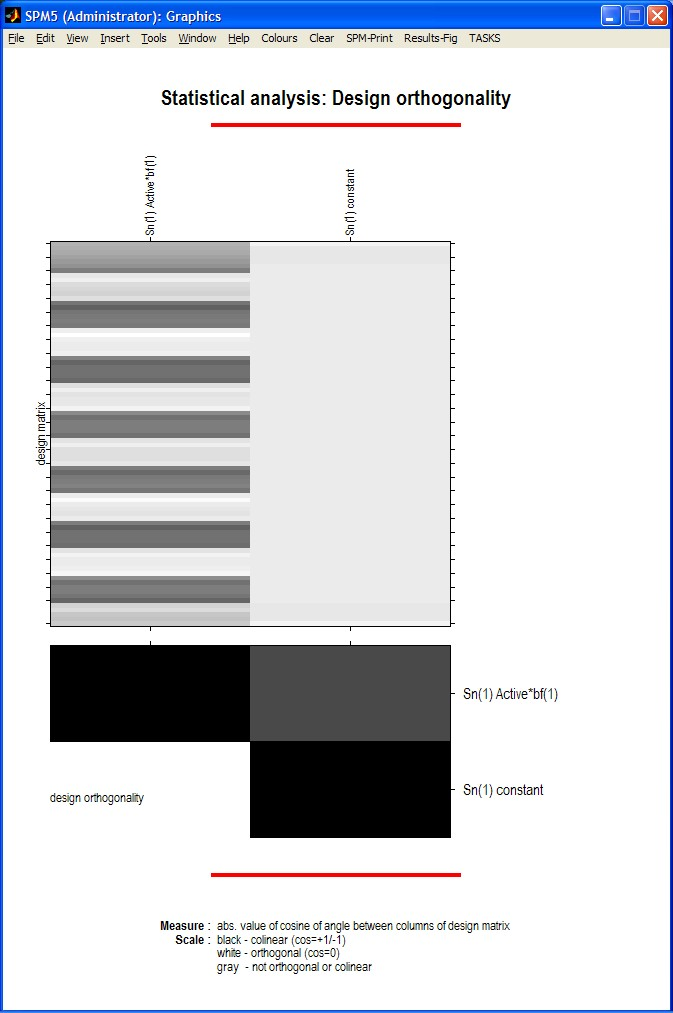
\includegraphics[width=80mm]{auditory/aud_orth}
\caption{\emph{\texttt{Design Orthogonality}: The description above the first column in the design matrix {\sf Sn(1)Active*bf(1)} means that this column refers to the first session of data (in this analysis there is only 1 session), the name of this condition/trial is `Active' and the trial information has been convolved with the first basis function (the canonical hemodynamic response). The constant regressor for session 1 is referred to as {\sf Sn(1)Constant}. The orthogonality matrix at the bottom indicates a degree of collinearity between regressors. \label{aud_orth}}}
\end{center}
\end{figure}

\subsection{Estimate}

Press the \textsc{Estimate} button. This will call up the specification of an fMRI estimation job in the batch editor. Then

\begin{itemize}
\item Highlight the ``Select SPM.mat'' option and then choose the \texttt{SPM.mat} file saved in the classical subdirectory.
\item Save the job as \texttt{estimate.job} and press the \texttt{Run} button.
\end{itemize}

SPM will write a number of files into the selected directory including an \texttt{SPM.mat} file.

\section{Inference}

After estimation:

\begin{itemize}
\item Press ``Results''.
\item Select the \texttt{SPM.mat} file created in the last section.
\end{itemize}

\begin{figure}
\begin{center}
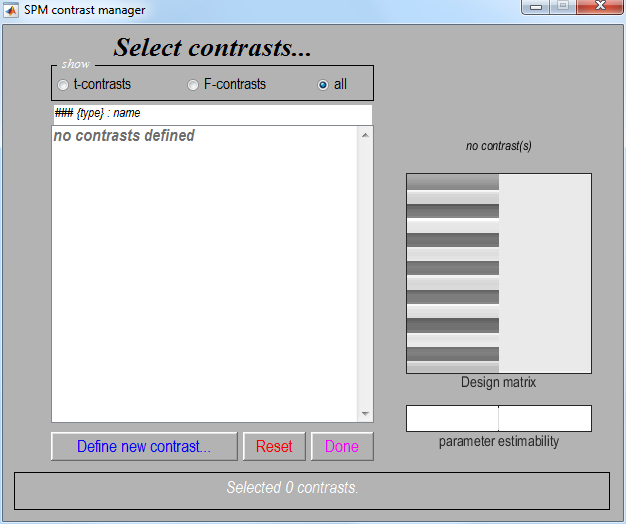
\includegraphics[width=60mm]{auditory/con_man}
\caption{\emph{The contrast manager}}
\end{center}
\end{figure}

This will invoke the contrast manager.

\subsection{Contrast manager}

The contrast manager displays the design matrix (surfable) in the right panel and lists specified contrasts in the left panel. Either ``t-contrast'' or ``F-contrast'' can be selected. To examine statistical results for condition effects

\begin{itemize}
\item{Select ``Define new contrast''}
\end{itemize}
\begin{figure}
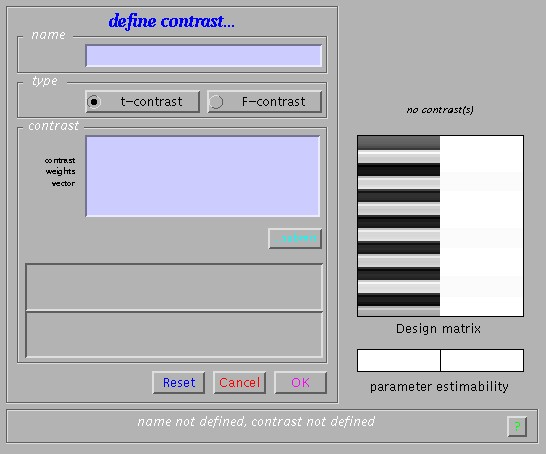
\includegraphics[width=60mm]{auditory/con_man2}
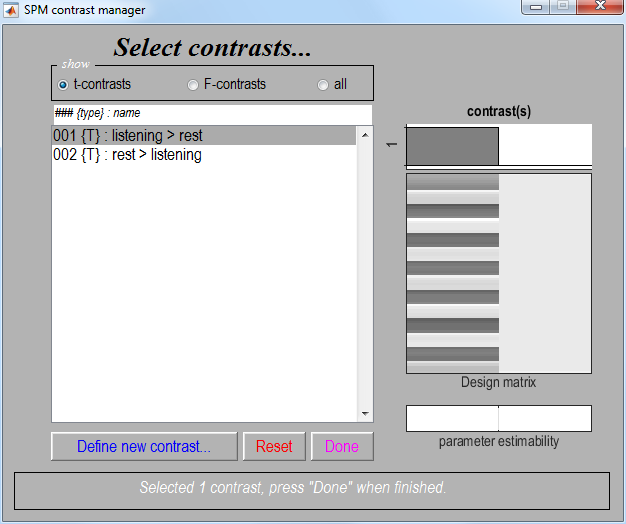
\includegraphics[width=60mm]{auditory/con_man3}
\caption{\emph{Left: A contrast is entered by specifying the numeric values in the lower window and the name in the upper window. Right: After contrasts have been specified they can be selected.}}
\end{figure}

One sided main effects for the active condition (i.e., a one-sided t-test) can be specified (in this example) as ``1'' (active $>$ rest) and ``-1'' (rest $>$ active). SPM will accept correct contrasts only. Accepted contrasts are displayed at the bottom of the contrast manager window in green, incorrect ones are displayed in red. To view a contrast

\begin{itemize}
\item Select the contrast name e.g., ``active $>$ rest''.
\item Press ``Done''.
\end{itemize}

\subsection{Masking}

You will then be prompted with

\begin{itemize}
\item  \emph{Mask with other contrast ? [Yes/No]}.
\item ``Specify No''.
\end{itemize}

Masking implies selecting voxels specified by other contrasts. If ''yes'', SPM will prompt for (one or more) masking contrasts, the significance level of the mask (default p = 0.05 uncorrected), and will ask whether an inclusive or exclusive mask should be used. Exclusive will remove all voxels which reach the default level of significance in the masking contrast, inclusive will remove all voxels which do not reach the default level of significance in the masking contrast. Masking does not affect p-values of the ''target'' contrast, it only includes or excludes voxels.

\subsection{Thresholds}

You will then be prompted with

\begin{itemize}
\item \emph{Title for comparison ?}
\item Enter eg. ``active  $>$ rest''.
\item \emph{p value adjustment to control: [FWE/FDR/none]}.
\item Select ``FWE''.
\item \emph{p value(family-wise error)}.
\item Accept the default value, 0.05.
\end{itemize}

A Family Wise Error (FWE) is a false positive anywhere in the SPM. Now, imagine repeating your experiment many times and producing SPMs. The proportion of SPMs containing FWEs is the FWE rate. A value of 0.05 implies that 1 in 20 SPMs contains a false positive somewhere in the image. 

If you choose the ``none'' option above this corresponds to making statistical inferences at the ``voxel level''. These use ``uncorrected'' p values, whereas FWE thresholds are said to use ``corrected'' p values. SPM's default uncorrected p value is p=0.001. This means that the probability of a false positive at each voxel is 0.001. So if, you have 50,000 voxels you can expect $50,000 \times 0.001 = 50$ false positives in each SPM.

%The final option here is False Discovery Rate (FDR). If you set this at 0.1, this means that of all the discoveries you make (ie. above threshold voxels that appear in the SPM) 10\% of them are likely to be false. 

You will then be prompted with

\begin{itemize}
\item \emph{Extent Threshold \{voxels\} [0]}.
\item Accept the default value, ``0''.
\end{itemize}

Entering a value $v$ here will produce SPMs with clusters containing at least $v$ voxels. SPM will then produce the SPM shown in Figure~\ref{aud_spm1}.

\begin{figure}
\begin{center}
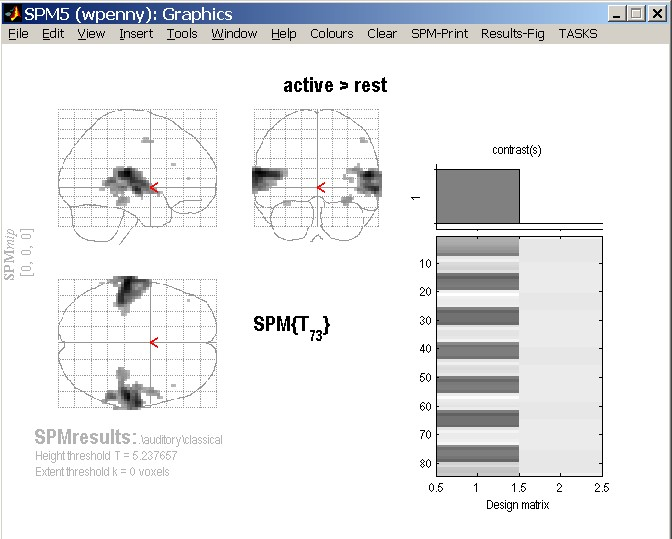
\includegraphics[width=100mm]{auditory/spm1}
\caption{\em SPM showing bilateral activation of auditory cortex. \label{aud_spm1}}
\end{center}
\end{figure}

\subsection{Files}

A number of files are written to the working directory at this time.
Images containing weighted parameter estimates are saved as \texttt{con\_0002.hdr/img}, \texttt{con\_0003.hdr/img}, etc. in the working directory. Images of T-statistics are saved as \texttt{spmT\_0002.hdr/img}, \texttt{spmT\_0003.hdr/img} etc., also in the working directory.

\subsection{Maximum Intensity Projections}

SPM displays a Maximum Intensity Projection (MIP) of the statistical map in the graphics window. The MIP is projected on a glass brain in three orthogonal planes. The MIP is surfable: right-clicking in the MIP will activate a pulldown menu, left-clicking  on the red cursor will allow it to be dragged to a new position.

\begin{figure}
\begin{center}
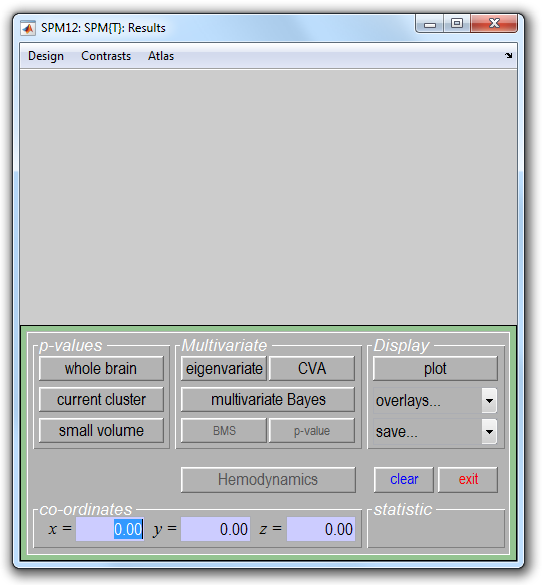
\includegraphics[width=100mm]{auditory/interactive}
\caption{\em SPM's Interactive window during results assessment. The ``p-values'' section is used to produce tables of statistical information. The visualisation section is used to plot responses at a voxel or to visual activations overlaid on anatomical images. The ``Multivariate'' section, ie. the ``eigenvariate'' button, is used to extract data for subsequent analyses such as assessment of PsychoPhysiological Interactions (PPIs) or Dynamic  Causal Models (DCMs).}
\end{center}
\end{figure}

\subsection{Design matrix}

SPM also displays the design matrix with the selected contrast. The design matrix is also surfable: right-clicking will show parameter names, left-clicking will show design matrix values for each scan. 

In the SPM Interactive window (lower left panel) a button box appears with various options for displaying statistical results (p-values panel) and creating plots/overlays (visualisation panel). Clicking ``Design'' (upper left) will activate a pulldown menu as in the ``Explore design'' option.

\subsection{Statistical tables}

To get a summary of local maxima, press the ``whole brain'' button in the p-values section of the interactive window. This will list all clusters above the chosen level of significance as well as separate ($>$8mm apart) maxima within a cluster, with details of significance thresholds and search volume underneath, as shown in Figure~\ref{aud_volume}

\begin{figure}
\begin{center}
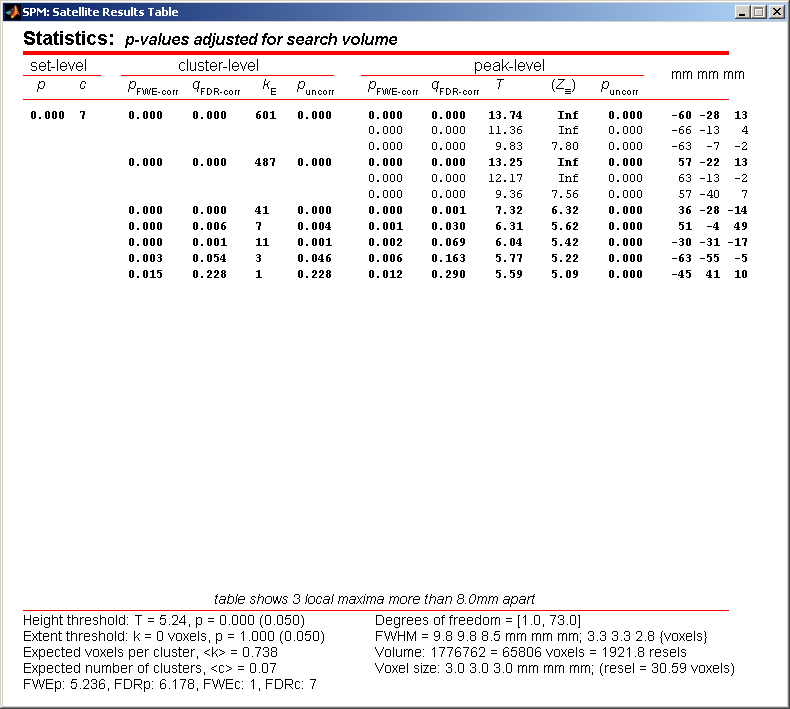
\includegraphics[width=100mm]{auditory/volume}
\caption{\em Volume table for ``active $>$ rest'' effect. This table of values was created by pressing the ``Results-Fig'' tab at the top of the graphics window and then pressing the ``whole brain'' button. This displays the table of results in a separate window. \label{aud_volume}}
\end{center}
\end{figure}

The columns in volume table show, from right to left:

\begin{itemize}
\item \textbf{x, y, z (mm)}: coordinates in MNI space for each maximum.
\item peak-level: the chance (p) of finding (under the null hypothesis) a peak with this or a greater height (T- or Z-statistic), corrected (FWE or FDR)/ uncorrected for search volume.
\item \textbf{cluster-level}: the chance (p) of finding a cluster with this many (ke) or a greater number of voxels, corrected (FWE or FDR)/ uncorrected for search volume.
\item \textbf{set-level}: the chance (p) of finding this (c) or a greater number of clusters in the search volume.
\end{itemize}

It is also worth noting that:

\begin{itemize}
\item The table is surfable: clicking a row of cluster coordinates will move the pointer in the MIP to that cluster, clicking other numbers will display the exact value in the \matlab\ window (e.g. 0.000 = 6.1971e-07).
\item To inspect a specific cluster (e.g., in this example data set, the right auditory cortex), either move the cursor in the MIP (by left-clicking and dragging the cursor, or right-clicking the MIP background which will activate a pulldown menu).
\item Alternatively, click the cluster coordinates in the volume table, or type the coordinates in the co-ordinates section of the interactive window.
\end{itemize}

It is also possible to produce tables of statistical information for a single cluster of interest rather than for the whole volume. Firstly, select the relevant cluster in the MIP and then press the ``current cluster'' button in the p-values section of the interactive window. This will show coordinates and voxel-level statistics for local maxima ($>$4mm apart) in the selected cluster. This table is also surfable.

\subsection{Plotting responses at a voxel}

A voxel can be chosen with co-ordinates corresponding to those in the interactive window. The responses at this voxel can then be plotted using the ``Plot'' button in the visualisation section of the interactive window. This will provide you with five further options:

\begin{enumerate}
\item Contrast estimates and 90\% CI: SPM will prompt for a specific contrast (e.g., active$>$rest). The plot will show effect size and 90\% confidence intervals. See eg. Figure~\ref{aud_contrast}.
\item Fitted responses: Plots adjusted data and fitted response across session/subject. SPM will prompt for a specific contrast and provides the option to choose different ordinates (``an explanatory variable'', ``scan or time'', or ``user specified''). If ``scan or time'', the plot will show adjusted or fitted data with errors added as shown in Figure~\ref{aud_fitted}.
\item Event-related responses: Plots adjusted data and fitted response across peri-stimulus time.
\item Parametric responses.
\item Volterra kernels.
\end{enumerate}

\begin{figure}
\begin{center}
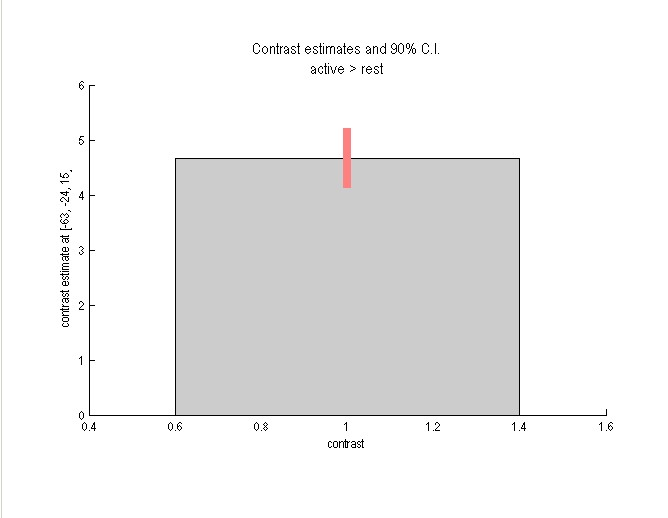
\includegraphics[width=60mm]{auditory/contrast}
\caption{\em Estimated effect size. \label{aud_contrast}}
\end{center}
\end{figure}

\begin{figure}
\begin{center}
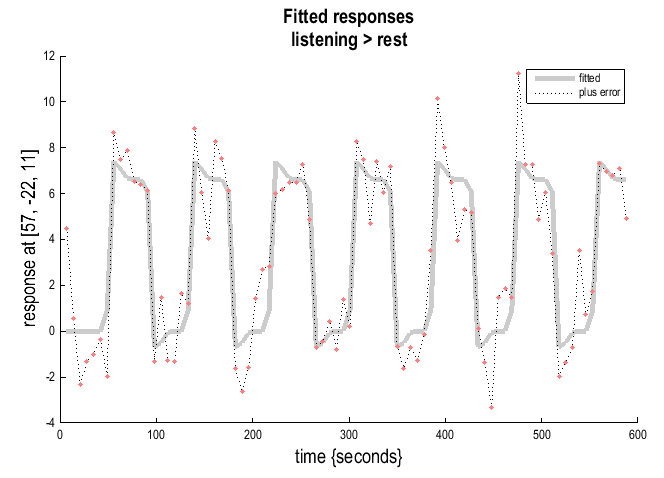
\includegraphics[width=60mm]{auditory/fitted}
\caption{\em Fitted responses. \label{aud_fitted}}
\end{center}
\end{figure}

For plotting event-related responses SPM provides three options

\begin{enumerate}
\item Fitted response and PSTH (peri-stimulus time histogram): plots mean regressor(s) (ie. averaged over session) and mean signal +/- SE for each peri-stimulus time bin.
\item Fitted response and 90\% CI: plots mean regressor(s) along with a 90\% confidence interval.
\item Fitted response and adjusted data: plots regressor(s) and individual data (note that in this example the data are shown in columns due to the fixed TR/ISI relationship).
\end{enumerate}

Its worth noting that

\begin{itemize}
\item The values for the fitted response across session/subject for the selected plot can be displayed and accessed in the Matlab window by typing ``Y''. Typing ``y'' will display the adjusted data.
\item ``Adjusted'' data = adjusted for confounds (e.g., global flow) and high- and low pass filtering.
\end{itemize}

\subsection{Overlays}

The visualisation section of the interactive window also provides an overlay facility for anatomical visualisation of clusters of activation. Pressing ``Overlays'' will activate a pulldown menu with three options

\begin{enumerate}
\item \textbf{Slices}: overlay on three adjacent (2mm) transaxial slices. SPM will prompt for an image for rendering. This could be a canonical image (see \texttt{spm\_template.man}) or an individual T1/mean EPI image for single-subject analyses.
\item \textbf{Sections}: overlay on three intersecting (sagittal, coronal, transaxial) slices. These renderings are surfable: clicking the images will move the crosshair.
\item \textbf{Render}: overlay on a volume rendered brain, with options for using a smoothed brain, and old (left) and new (right) style rendering.
\end{enumerate}

Renderings can be saved as \texttt{filename.img/hdr} in the working directory by using the {\em write filtered} option. In Figures~\ref{aud_slices}, \ref{aud_sections} and \ref{aud_render} the `active $>$ rest' activation has been superimposed on the spatially normalised, bias-corrected anatomical image \texttt{wmsM00223\_002.img} created earlier. 

\begin{figure}
\begin{center}
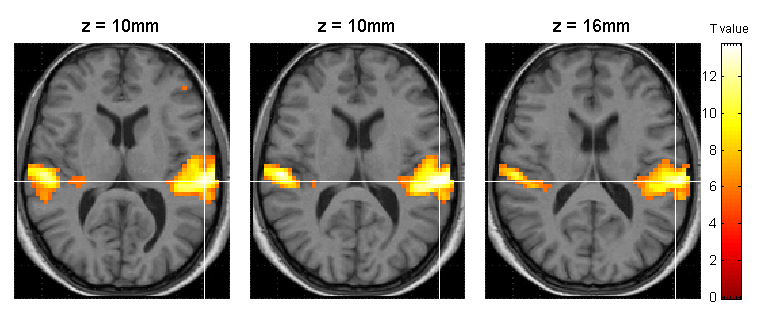
\includegraphics[width=100mm]{auditory/slices}
\caption{\emph{Slices.} \label{aud_slices} }
\end{center}
\end{figure}

\begin{figure}
\begin{center}
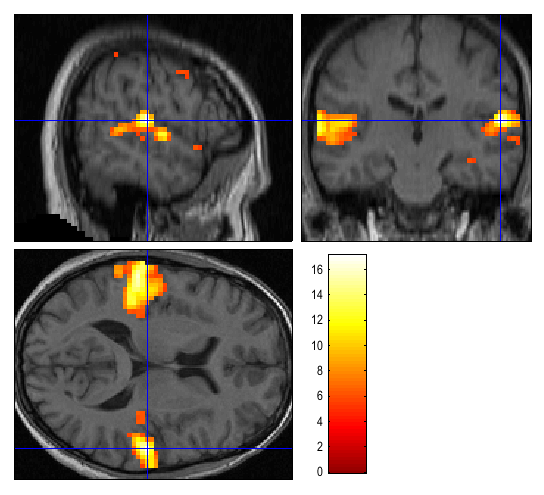
\includegraphics[width=100mm]{auditory/sections}
\caption{\emph{Sections.} \label{aud_sections} }
\end{center}
\end{figure}

For the ``Render'' option we first created a rendering for this subject. This was implemented by 

\begin{itemize}
\item ``Normalise (Write)'' the two images \texttt{c1sM00223\_002.img} and \texttt{c2sM00223\_002.img} using the ``Parameter File '' \texttt{sM00223\_002\_seg\_sn.mat} and a voxel size of [1 1 3].
\item Selecting ``Xtract Surface'' from the ``Render'' pulldown menu.
\item Selecting the gray and white matter images \texttt{wc1sM00223\_002.img} and \texttt{wc2sM00223\_002.img} created in the first step.
\item Saving the results using the default options (Rendering and Surface).
\end{itemize}

SPM plots the rendered anatomical image in the graphics window and saves it as \texttt{render\_wc1sM00223\_002.mat}. The surface image is saved as \texttt{surf\_wc1sM00223\_002.mat}).

\begin{figure}
\begin{center}
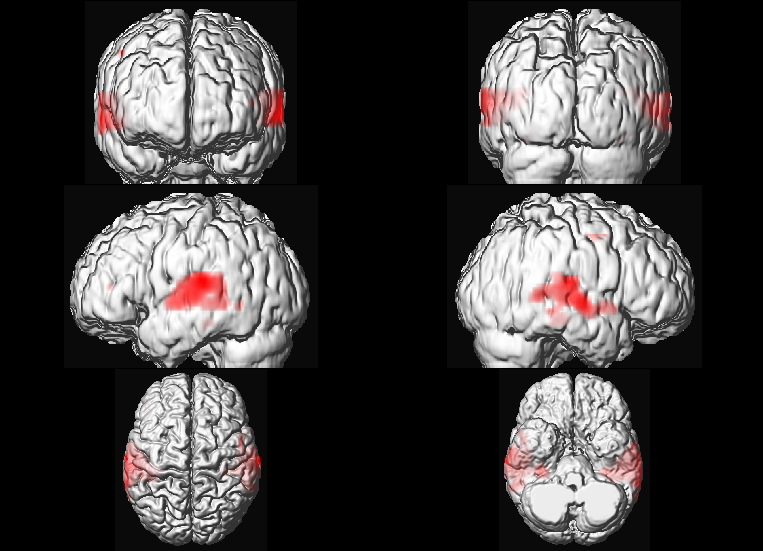
\includegraphics[width=100mm]{auditory/render}
\caption{\emph{Render.} \label{aud_render} }
\end{center}
\end{figure}

\subsection{Miscellaneous}

Other options (in the results controls panel):

\begin{itemize}
\item \textbf{clear}: clears lower subpanel of Graphics window,
\item \textbf{exit}: exits the results section,
\item \textbf{?}: launches help.
\end{itemize}

\section{Bayesian analysis}

\subsection{Specification}

Press the ``Specify 1st-level'' button. This will call up an fMRI specification job in the batch editor. Then

\begin{itemize}
\item Open the fMRI model specification option.
\item Load the ``specify.mat'' job file created for the classical analysis.
\item Open ``Subject/Session'', highlight ``Scans''.
\item Deselect the smoothed functional images using the ``unselect all'' option available from a right mouse click in the SPM file selector (bottom window).
\item Select the unsmoothed functional images using the \texttt{\^w.*} filter and `select all' option available from a right mouse click in the SPM file selector (top right window)\footnote{Remember not to select the first 12 scans, scans 4 to 15, as these may contain T1 effects. This can be done during selection or by first moving the files to a different directory.}. The Bayesian analysis uses a spatial prior where the spatial regularity in the signal is estimated from the data. It is therefore not necessary to create smoothed images if you are only going to do a Bayesian analysis.
\item Press ``Done''.
\item Highlight ``Directory'' and select the \texttt{DIR/bayesian} directory you created earlier (you will first need to deselect the \texttt{DIR/classical} directory).
\item Save the job as \texttt{specify\_bayesian.mat} and press the ``Run'' button.
\end{itemize}

\subsection{Estimation}

Press the ``Estimate'' button. This will call up the specification of an fMRI estimation job in the batch editor. Then

\begin{itemize}
\item Highlight the ``Select SPM.mat'' option and then choose the SPM.mat file saved in the \texttt{DIR/bayesian} directory.
\item Highlight ``Method'' and select the ``Choose Bayesian 1st-level'' option.
\item Open the newly created ``Bayesian 1st-level'' option, highlight ``AR model order'' and select 0. This data set has a TR=7s, so is unlikely to have temporally autocorrelated errors.
\item Save the job as \texttt{estimate\_bayesian.job} and press the ``Run'' butto.
\end{itemize}

SPM will write a number of files into the output directory including 

\begin{itemize}
\item An \texttt{SPM.mat} file.
\item Images of estimated regression coefficients  \texttt{Cbeta\_0001.img} and \texttt{Cbeta\_0002.img}. These filenames are prefixed with a \texttt{C} indicating that these are the mean values of the ``Conditional'' or ``Posterior'' density.
\item Images of error bars/standard deviations on the regression coefficients \texttt{SDbeta\_0001.img} and \texttt{SDbeta\_0002.img}.
\item An image of the standard deviation of the error \texttt{Sess1\_SDerror.img}.
\item An image \texttt{mask.img} indicating which voxels were included in the analysis.
\end{itemize}

\subsection{Inference}

After estimation:

\begin{itemize}
\item Press ``Results'',
\item Select the \texttt{SPM.mat} file created in the last section,
\item Select ``Define new contrast'',
\item Enter the name ``active $>$ rest'',
\item Enter the value ``1'', press ``Submit'', ``OK'', ``Done'',
\item \emph{Mask with other contrast ? [Yes/No]},
\item Specify No,
\item Title for comparison, accept the default,
\item \emph{Effect size threshold for PPM},
\item Enter the value 2,
\item \emph{Posterior probability threshold for PPM},
\item Enter the value 0.99,
\item \emph{Extent threshold [0]},
\item Accept the default value,
\item \emph{Plot effect size [Yes/No]},
\item Select the default `Yes'.
\end{itemize}

SPM will then plot a map of effect sizes at voxels where it is 99\% sure that the effect size is greater than 2\% of the global mean. This is a large activation. Then use overlays, sections, select the normalised structural image created earlier and move the cursor to the activation in the left hemisphere. This should create the plot shown in Figure~\ref{aud_bayes}.

\begin{figure}
\begin{center}
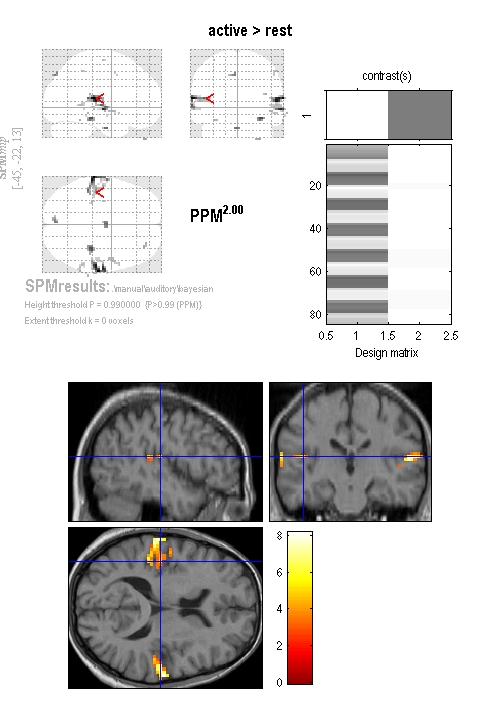
\includegraphics[width=100mm]{auditory/aud_bayes}
\caption{\em \textbf{Bayesian analysis:} MIP and overlay of effect sizes at voxels where SPM is 99\% sure that the effect size is greater than 2\% of the global mean. \label{aud_bayes} }
\end{center}
\end{figure}

It is also possible to look for regions where responses in the active condition are different to those at rest. Active responses could be greater or smaller.

\begin{itemize}
\item Press ``Results'',
\item Select the \texttt{SPM.mat} file created in the last section,
\item Select ``Define new contrast'' and highlight the ``F'' radio button,
\item Enter the name ``active != rest'',
\item Enter the value ``1'', press ``Submit'', ``OK'', ``Done'',
\item \emph{Mask with other contrast ? [Yes/No]},
\item Specify ``No'',
\item Title for comparison, accept the default,
\item \emph{Posterior probability threshold for PPM},
\item Accept the default value\footnote{The default PPM threshold is set to $1-1/S$ where S is the number of voxels in the volume being analysed. The rationale for this is that inference is based on an approximate posterior distribution, $Q$, which factorises across voxels. The approximate posterior is chosen to best match the true posterior in the sense of KL-divergence. Given the factorisation in $Q$, the expected number of false positives in the PPM is 1. },
\item \emph{Extent threshold [0]},
\item Accept the default value, 0,
\item \emph{Plot effect size [Yes/No]},
\item Select the default ``Yes''.
\end{itemize}

SPM will then plot a map of $\chi^2$ statistic values at above threshold voxels. Then use overlays, sections, select the normalised structural image created earlier and move the cursor to the activation in the left hemisphere. This should create the plot shown in Figure~\ref{aud_bayes2}

\begin{figure}
\begin{center}
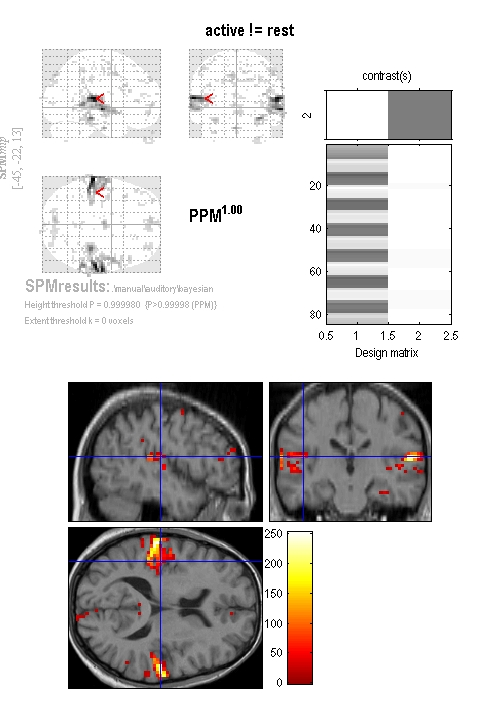
\includegraphics[width=100mm]{auditory/aud_bayes2}
\caption{\em \textbf{Two-sided Bayesian analysis:} MIP and overlay of $\chi^2$ statistic values at above threshold voxels. This shows regions where activity is different between active and rest conditions, whether positive or negative. \label{aud_bayes2} }
\end{center}
\end{figure}

When you revisit the contrast manager this contrast will be referred to as a ``P'' contrast, rather than an ``F'' contrast. This indicates that Bayes rule is used to make the inference. To indicate that we are testing a two-sided effect it is advisable to make this clear when naming the contrast (as we have done with the label ``active != rest'').


\chapter{Face data \label{Chap:data:faces}}

As another, more sophisticated example, consider the data from a repetition priming experiment performed using event-related fMRI.
Briefly, this is a 2$\times$2 factorial study with factors ``fame'' and ``repetition'' where famous and non-famous faces were presented twice against a checkerboard baseline (for more details, see \cite{rnah_face_rep}). The subject was asked to make fame judgements by making key presses. There are thus four event-types of interest; first and second presentations of famous and non-famous faces, which we denote N1, N2, F1 and F2. The experimental stimuli and timings of events are shown in Figures~\ref{face_stim} and \ref{face_timing}.

\begin{figure}
\begin{center}
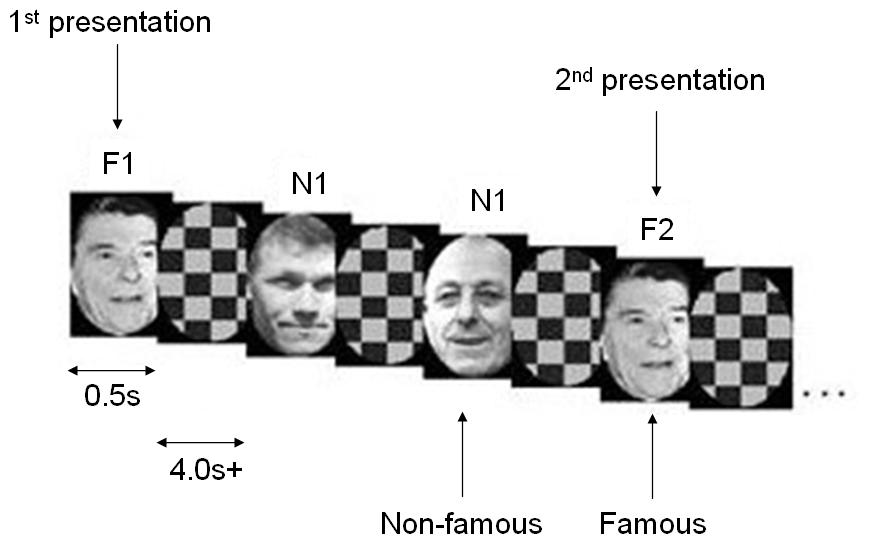
\includegraphics[width=120mm]{faces/face_stim}
\caption{\em \textbf{Face repetition paradigm}: There were 2 presentations of 26 Famous and 26 Nonfamous Greyscale photographs, for 0.5s each, randomly intermixed. The minimal Stimulus Onset Asynchrony (SOA)=4.5s, with probability 2/3 (ie 1/3 null events). The subject made one of two right finger key presses denoting whether or not the subject thought the face was famous. \label{face_stim}}
\end{center}
\end{figure}

\begin{figure}
\begin{center}
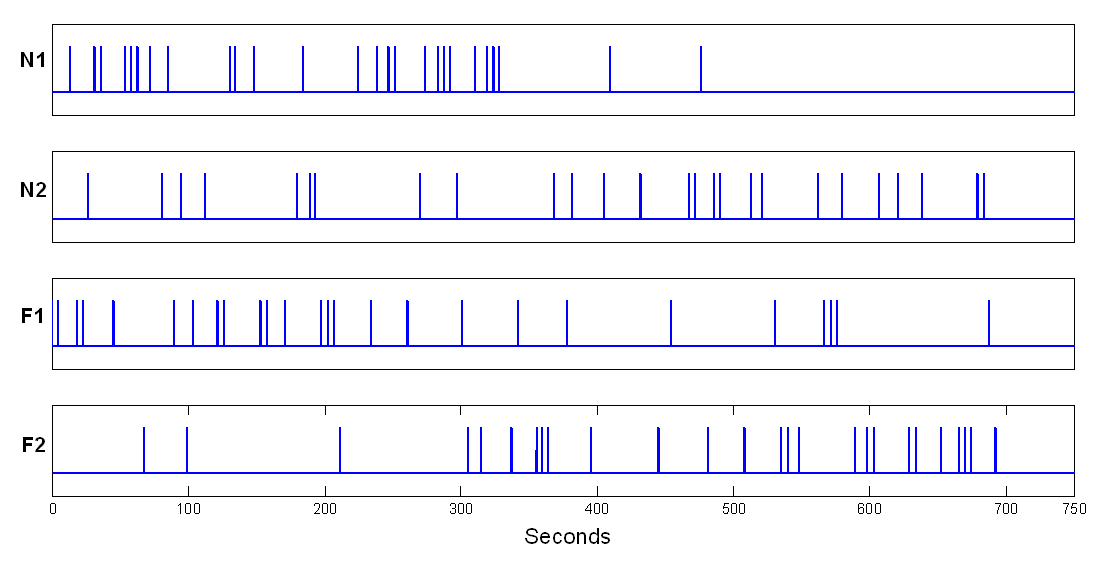
\includegraphics[width=140mm]{faces/face_timing}
\caption{\em Time series of events. \label{face_timing}}
\end{center}
\end{figure}

Images were acquired using continuous Echo-Planar Imaging (EPI) with TE=40ms, TR=2s and 24 descending slices (64$\times$64 3$\times$3 mm$^2$), 3mm thick with a 1.5mm gap.
The data archive is available from the SPM website\footnote{Face Repetition dataset: \url{http://www.fil.ion.ucl.ac.uk/spm/data/face_rep/}}.
This contains 351 Analyze format functional images \texttt{sM03953\_0005\_*.img} of dimension 64$\times$64$\times$24 with 3$\times$3$\times$4.5 mm$^3$ voxels. A structural image is also provided  in Analyze format (\texttt{sM03953\_0007.img}).

To analyse the data, first create a new directory \texttt{DIR} eg. \texttt{C:$\backslash$data$\backslash$face\_rep}, in which to place the results of your analysis. Then create 4 subdirectories (i) \texttt{jobs}, (ii) \texttt{categorical}, (iii)  \texttt{parametric} and (iv) \texttt{bayesian}. As the analysis proceeds these directories will be filled with job-specification files, design matrices and models estimated using classical or Bayesian methods. 

As well as the classical/Bayesian distinction we will show how this data can be analysed from a parametric as well as a categorical perspective. We will look at the 
main effects of fame and repetition and in the parameteric analysis we will look at responses as a function of ``lag'', that is, the number of faces intervening between repetition of a specific face.

Start up matlab, enter your jobs directory and type \texttt{spm fmri} at the \matlab\ prompt. SPM will then open in fMRI mode with three windows (1) the top-left or ``Menu'' window, (2) the bottom-left or ``Interactive'' window and (3) the right-hand or ``Graphics'' window. 
Analysis then takes place in three major stages (i) spatial pre-processing, (ii) model specification, review and estimation and (iii) inference. These stages organise the buttons in SPM's base window.
\begin{figure}
\begin{center}
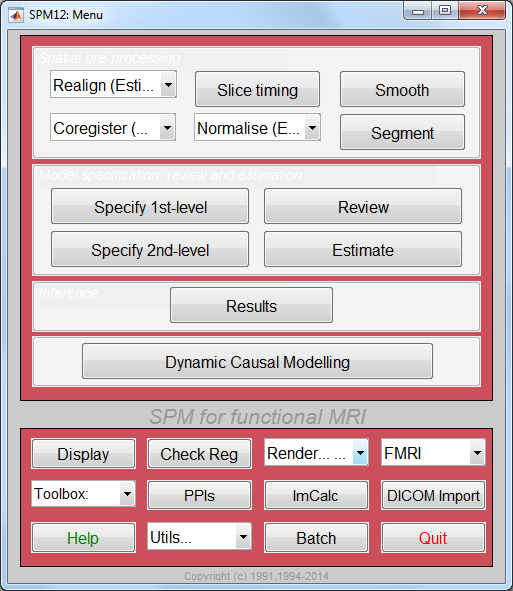
\includegraphics[width=100mm]{faces/command}
\caption{\em The SPM base window comprises three sections (i) spatial pre-processing, (ii) model specification, review and estimation and (iii) inference. \label{command}}
\end{center}
\end{figure}

\section{Spatial pre-processing}

\subsection{Display}

Display eg. the first functional image using the ``Display'' button. Note orbitofrontal and inferior temporal drop-out and ghosting. This can be seen more clearly by selecting ``brighten'' from the ``Effects'' tab in the ``Colours'' at the top of the Graphics window.

\begin{figure}
\begin{center}
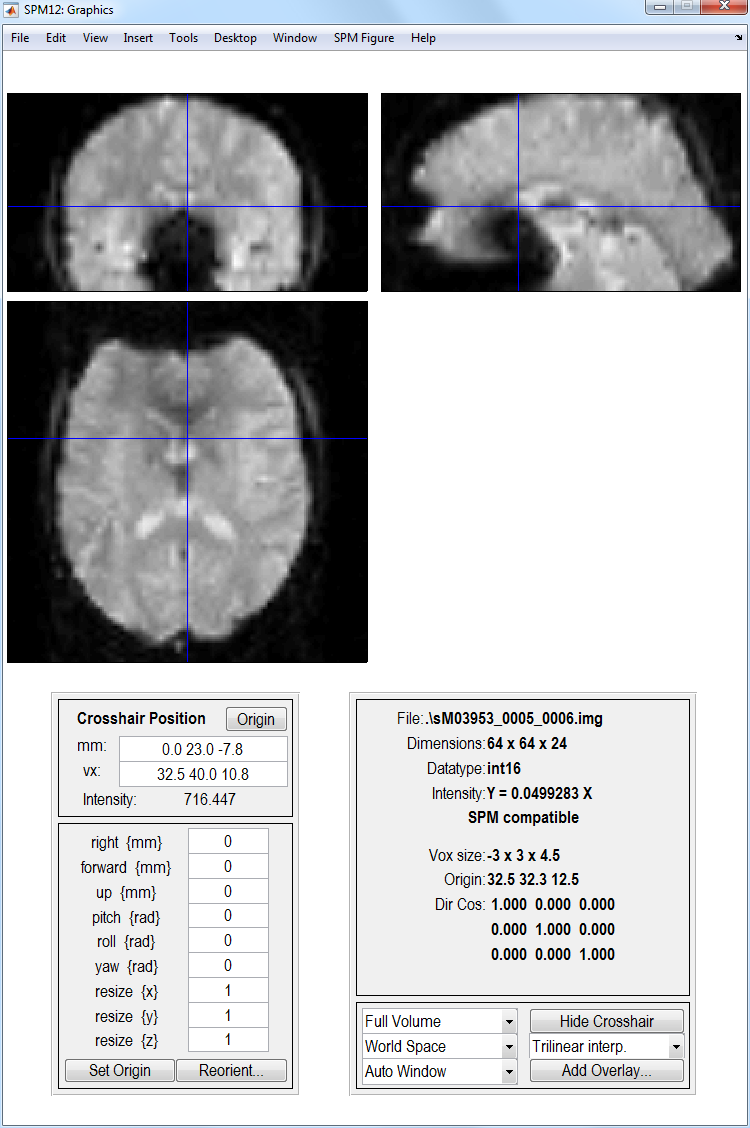
\includegraphics[width=100mm]{faces/dropout}
\caption{\em Signal dropout in EPI images. \label{dropout}}
\end{center}
\end{figure}

\subsection{Realignment}

Under the spatial pre-processing section of the SPM base window select \textsc{Realign (Est \& Res)} from the \textsc{Realign} pulldown menu. This will call up a realignment job specification in the batch editor window.
Then
\begin{itemize}
\item Highlight data, select ``New Session'', then highlight the newly created ``Session'' option.
\item Select ``Specify Files'' and use the SPM file selector to choose all of your functional images eg. \texttt{sM03953\_0005\_*.img}.
\item Save the job file as eg. \texttt{DIR/jobs/realign.mat}.
\item Press the \texttt{Rrn} button in the batch editor window (green triangle).
\end{itemize}
This will run the realign job which will write realigned images into the directory where the functional images are. These new images will be prefixed with the letter ``\texttt{r}''. SPM will then plot the estimated time series of translations and rotations shown in Figure~\ref{face_realign}. These data, the realignment parameters, are also saved to a file eg. \texttt{rp\_sM03953\_0005\_0006.txt}, so that these variables can be used as regressors when fitting GLMs. To prepare for this, copy the file into the \texttt{DIR/jobs} directory and rename it \texttt{movepars.txt}. This allows movements effects to be discounted when looking for brain activations.

SPM will also create a mean image eg. \texttt{meansM03953\_0005\_0006.img} which will be used in the next step of spatial processing - coregistration.
\begin{figure}
\begin{center}
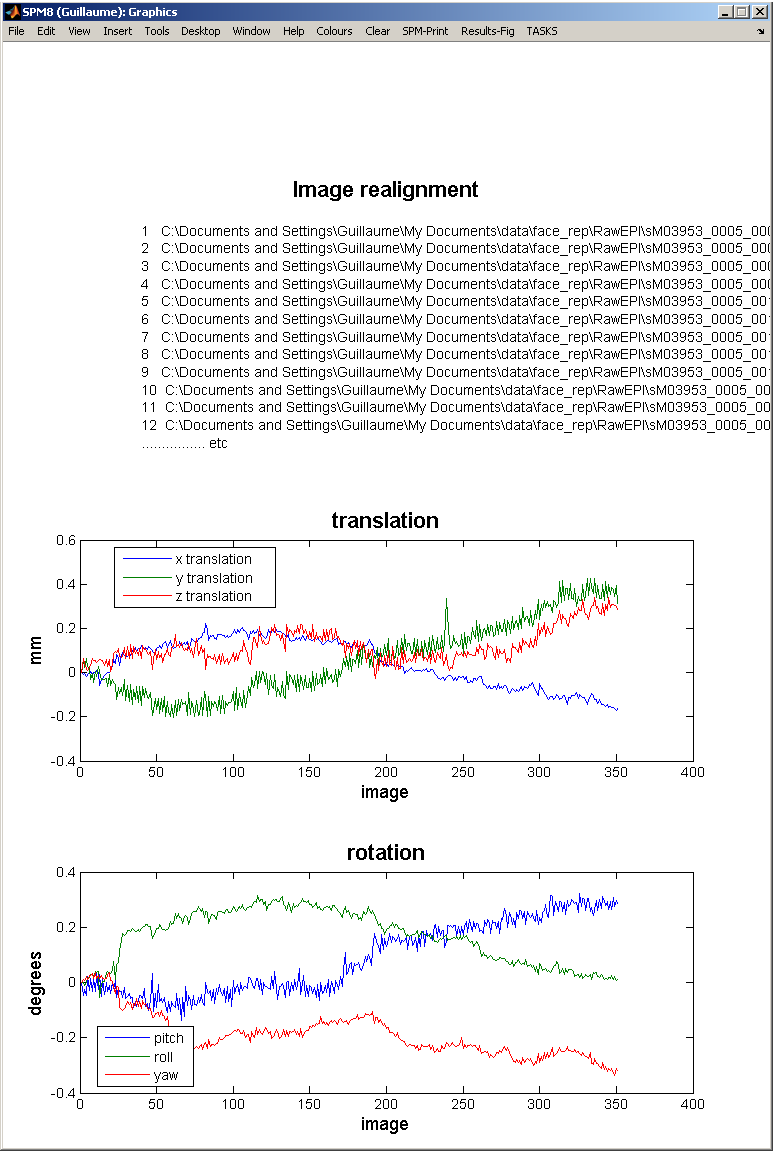
\includegraphics[width=100mm]{faces/realign}
\caption{\em \textbf{Realignment of face data}: Movement less than the size of a voxel, which for this data set is 3mm, is not considered problematic. \label{face_realign}}
\end{center}
\end{figure}

\subsection{Slice timing correction}

Press the textsc{Slice timing} button. This will call up the specification of a slice timing job in the batch editor window. Note that these data consist of N=24 axial slices acquired continuously with a TR=2s (ie TA = TR - TR/N, where TA is the time between the onset of the first and last slice of one volume, and the TR is the time between the onset of the first slice of one volume and the first slice of next volume) and in a descending order (ie, most superior slice was sampled first). The data however are ordered within the file such that the first slice (slice number 1) is the most inferior slice, making the slice acquisition order [24 23 22 ... 1].

\begin{itemize}
\item Highlight ``Data'' and select ``New Sessions''
\item Highlight the newly create ``Sessions'' option, ``Specify Files'' and select the 351 realigned functional images using the filter \texttt{\textasciicircum r.*}.
\item Select ``Number of Slices'' and enter 24.
\item Select TR and enter 2.
\item Select TA and enter 1.92 (or 2 - 2/24).
\item Select ``Slice order'' and enter 24:-1:1.
\item Select ``Reference Slice'', and enter 12.
\item Save the job as \texttt{slice\_timing.mat} and press the ``Run'' button.
\end{itemize}
SPM will write slice-time corrected files with the prefix ``\texttt{a}'' in the functional data directory.

\subsection{Coregistration}

Select \textsc{Coregister (Estimate)} from the \texttt{Coregister} pulldown menu. This will call up the specification of a coregistration job in the batch editor 
window. 

\begin{itemize}
\item Highlight ``Reference Image'' and then select the mean functional image \texttt{meansM03953\_0005\_0006.img}.
\item Highlight ``Source Image'' and then select the structural image eg. \texttt{sM03953\_0007.img}.
\item Press the ``Save'' button and save the job as \texttt{coreg.job}
\item Then press the ``Run'' button.
\end{itemize}

SPM will then implement a coregistration between the structural and functional data that maximises the mutual information. The image in figure~\ref{face_coreg} should then appear in the graphics window. SPM will have changed the header of the source file which in this case is the structural image \texttt{sM03953\_0007.img}.

\begin{figure}
\begin{center}
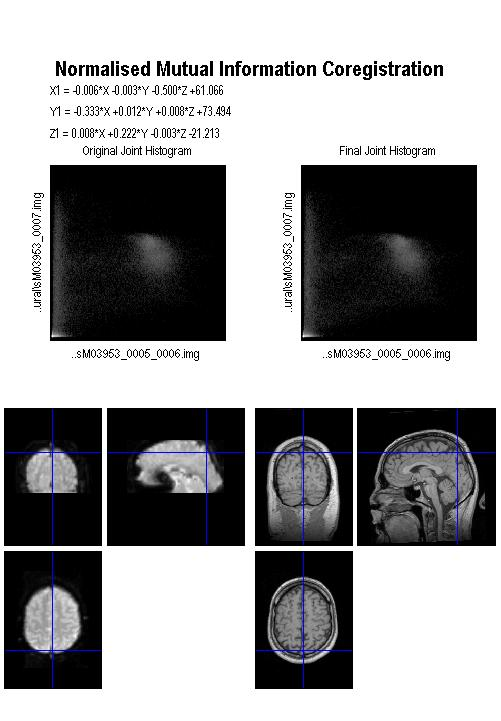
\includegraphics[width=100mm]{faces/coreg}
\caption{\em Mutual Information Coregistration of Face data.\label{face_coreg}}
\end{center}
\end{figure}

\subsection{Segmentation}

Press the \textsc{Segment} button. This will call up the specification of a segmentation job in the batch editor window. Highlight the ``Data'' field and then select the subjects coregistered anatomical image eg. \texttt{sM03953\_0007.img}. Save the job file as \texttt{segment.mat} and then press the \texttt{Run} button. SPM will segment the structural image using the default tissue probability maps as priors. 
SPM will create, by default, gray and white matter images and bias-field corrected structral image. These can be viewed using the CheckReg facility as described in the previous section. Figure~\ref{face_gray} shows the gray matter image, \texttt{c1sM03953\_0007.img}, along with the original structural\footnote{Segmentation can sometimes fail if the source (structural) image is not close in orientation to the MNI templates. It is generally advisable to manually orient the structural to match the template (ie MNI space) as close as possible by using the ``Display'' button, adjusting x/y/z/pitch/roll/yaw, and then pressing the ``Reorient'' button.}.

\begin{figure}
\begin{center}
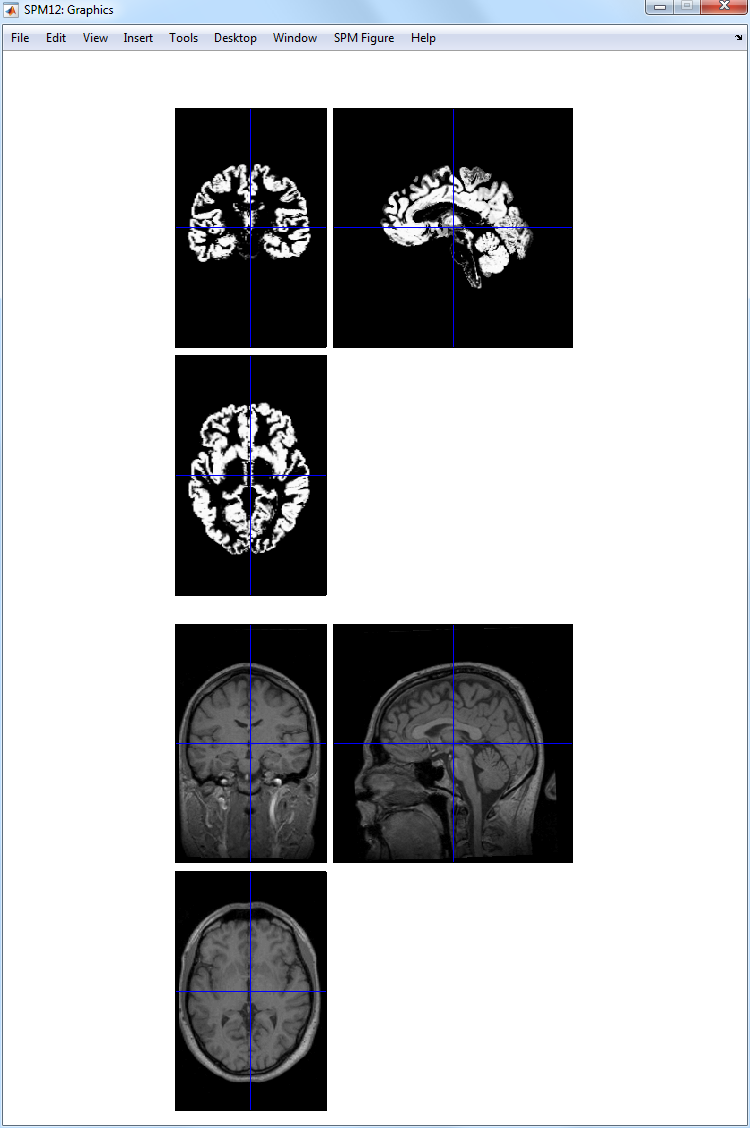
\includegraphics[width=100mm]{faces/gray}
\caption{\em Gray matter (top) produced by segmentation of structural image (below). \label{face_gray}}
\end{center}
\end{figure}

SPM will also write a spatial normalisation eg. \texttt{sM03953\_0007\_seg\_sn.mat} file in the original structural directory. This will be used in the next section to normalise the functional data. 

\subsection{Normalise}

Select \textsc{Normalise (Write)} from the \textsc{Normalise} pulldown menu. This will call up the specification of a normalise job in the batch editor window. 

\begin{itemize}
\item Highlight ``Data'', select ``New Subject''.
\item Open ``Subject'', highlight ``Parameter File'' and select the \texttt{sM03953\_0007\_seg\_sn.mat} file that you created in the previous section.
\item Highlight images to write and select all of the slice-time corrected, realigned functional images \texttt{arsM*.img}. Note: This can be done efficiently by changing the filter in the SPM file selector to \texttt{\textasciicircum ar.*}. You can then right click over the listed files, choose ``Select all''. You might also want to select the mean functional image created during realignment (which would not be affected by slice-time correction), i.e, the \texttt{meansM03953\_0005\_006.img}. Then press ``Done''.
\item Open ``Writing Options'', and change ``Voxel sizes'' from [2 2 2] to [3 3 3]\footnote{This step is not strictly necessary. It will write images out at a resolution closer to that at which they were acquired. This will speed up subsequent analysis and is necessary, for example, to make Bayesian fMRI analysis computationally efficient.}.
\item Press ``Save'', save the job as normalise.mat and then press the \texttt{Run} button.
\end{itemize}
SPM will then write spatially normalised files to the functional data directory. These files have the prefix ``\texttt{w}''.

If you wish to superimpose a subject's functional activations on their own anatomy\footnote{Beginners may wish to skip this step, and instead just superimpose functional activations on an ``canonical structural image''.} you will also need to apply the spatial normalisation parameters to their (bias-corrected) anatomical image. To do this
\begin{itemize}
\item Select \textsc{Normalise (Write)}, highlight `Data', select ``New Subject''.
\item Highlight ``Parameter File'', select the \texttt{sM03953\_0007\_seg\_sn.mat} file that you created in the previous section, press ``Done''.
\item Highlight ``Images to Write'', select the bias-corrected structural eg. \texttt{msM03953\_0007.img}, press ``Done''.
\item Open ``Writing Options'', select voxel sizes and change the default [2 2 2] to [1 1 1] which better matches the original resolution of the images [1 1 1.5].
\item Save the job as \texttt{norm\_struct.mat} and press \texttt{Run} button.
\end{itemize}

\subsection{Smoothing}

Press the \textsc{Smooth} button\footnote{The smoothing step is unnecessary if you are only interested in Bayesian analysis of your functional data.}. This will call up the specification of a smooth job in the batch editor window.

\begin{itemize}
\item Select ``Images to Smooth'' and then select the spatially normalised files created in the last section eg. \texttt{war*.img}.
\item Save the job as {\sf smooth.mat} and press \texttt{Run} button.
\end{itemize}

This will smooth the data by (the default) 8mm in each direction, the default smoothing kernel width.

\begin{figure}
\begin{center}
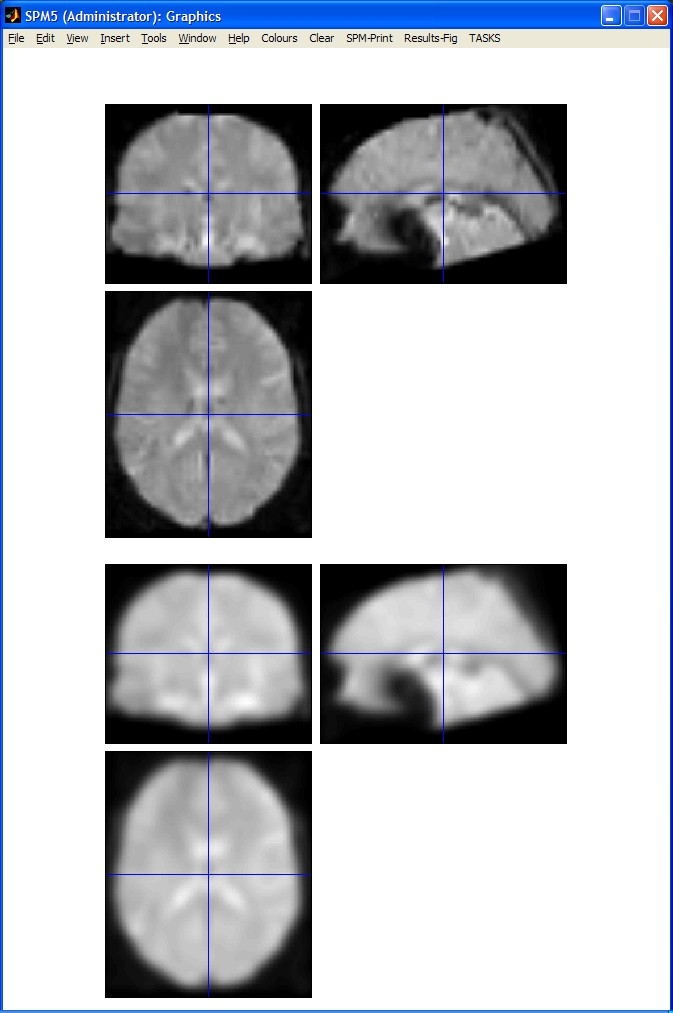
\includegraphics[width=100mm]{faces/smooth}
\caption{\em Functional image (top) and 8mm-smoothed functional image (bottom). These images were plotted using SPM's ``CheckReg'' facility. \label{face_smooth}}
\end{center}
\end{figure}

\section{Modelling categorical responses}

Before setting up the design matrix we must first load the Stimulus Onsets Times (SOTs) and movement parameters into matlab. SOTs are stored in the \texttt{sots.mat} file in a cell array such that eg. \texttt{sot\{1\}} contains stimulus onset times in TRs for event type 1, which is N1. Event-types 2, 3 and 4 are N2, F1 and F2.\footnote{Unlike previous analyses of these data in SPM99 and SPM2, we will not bother with extra event-types for the (rare) error trials.}
\begin{itemize}
\item At the \matlab\ command prompt type \texttt{load sots}
\item Then type \texttt{load movepars.txt}
\end{itemize}

Now press the \textsc{Specify 1st-level} button. This will call up the specification of a fMRI specification job in the batch editor window. Then

\begin{itemize}
\item In the ``Timing paramaters'' option,
\item Highlight ``Units for design'' and select ``Scans'',
\item Highlight ``Interscan interval'' and enter 2,
\item Highlight ``Microtime resolution'' and enter 24,
\item Highlight ``Microtime onset'' and enter 12. These last two options make the creating of regressors commensurate with the slice-time correction we have applied to the data, given that there are 24 slices and that the reference slice to which the data were slice-time corrected was the 12th (middle slice in time).
\item Highlight ``Data and Design'' and select ``New Subject/Session''.
\item Highlight ``Scans'' and use SPM's file selector to choose the 351 smoothed, normalised, slice-time corrected, realigned functional images ie \texttt{swarsM.img}. These can be selected easily using the \texttt{\textasciicircum swar.*} filter, and select all. Then press ``Done''.
\item Highlight ``Conditions'' and select ``New condition''\footnote{It is also possible to enter information about all of the conditions in one go. This requires much less button pressing and can be implemented by highlighting the ``Multiple conditions'' option and then selecting the \texttt{all-conditions.mat} file, which is also provided on the webpage.}.
\item Open the newly created ``Condition'' option. Highlight ``Name'' and enter ``N1''. Highlight ``Onsets'' and enter \texttt{sot\{1\}}. Highlight ``Durations'' and enter 0.
\item Highlight ``Conditions'' and select ``Replicate condition''.
\item Open the newly created ``Condition'' option (the lowest one). Highlight ``Name'' and change to ``N2''. Highlight ``Onsets'' and enter \texttt{sot\{2\}}.
\item Highlight ``Conditions'' and select ``Replicate condition''.
\item Open the newly created ``Condition'' option (the lowest one). Highlight ``Name'' and change to ``F1''. Highlight ``Onsets'' and enter \texttt{sot\{3\}}.
\item Highlight ``Conditions'' and select ``Replicate condition''.
\item Open the newly created ``Condition'' option (the lowest one). Highlight ``Name'' and change to ``F2''. Highlight ``Onsets'' and enter \texttt{sot\{4\}}.
\item Highlight ``Multiple Regressors'' and select the \texttt{movepars.txt} file\footnote{It is also possible to enter regressors one by one by highlighting ``Regressors'' and selecting ``New Regressor'' for each one. Here, we benefit from the fact that the realignment stage produced a text file with the correct number of rows (351) and columns (6) for SPM to add 6 regressors to model (linear) rigid-body movement effects.}.
\item Highlight ``Factorial Design'', select ``New Factor'', open the newly created ``Factor'' option, highlight ``Name'' and enter ``Fam'', highlight ``Levels'' and enter 2.
\item Highlight ``Factorial Design'', select ``New Factor'', open the newly created ``Factor'' option, highlight ``Name'' and enter ``Rep'', highlight ``Levels'' and enter 2\footnote{The order of naming these factors is important - the factor to be specified first is the one that ``changes slowest'' ie. as we go through the list of conditions N1, N2, F1, F2 the factor ``repetition'' changes every condition and the factor ``fame'' changes every other condition. So ``Fam'' changes slowest and is entered first.}.
\item Open ``Canonical HRF'' under ``Basis Functions''. Select ``Model derivatives'' and select ``Time and Dispersion derivatives''.
\item Highlight ``Directory'' and select the \texttt{DIR/categorical} directory you created earlier.
\item Save the job as \texttt{categorical\_spec.mat} and press the \texttt{Run} button.
\end{itemize}

SPM will then write an \texttt{SPM.mat} file to the \texttt{DIR/categorical} directory. It will also plot the design matrix, as shown in Figure~\ref{cat_design}. 
\begin{figure}
\begin{center}
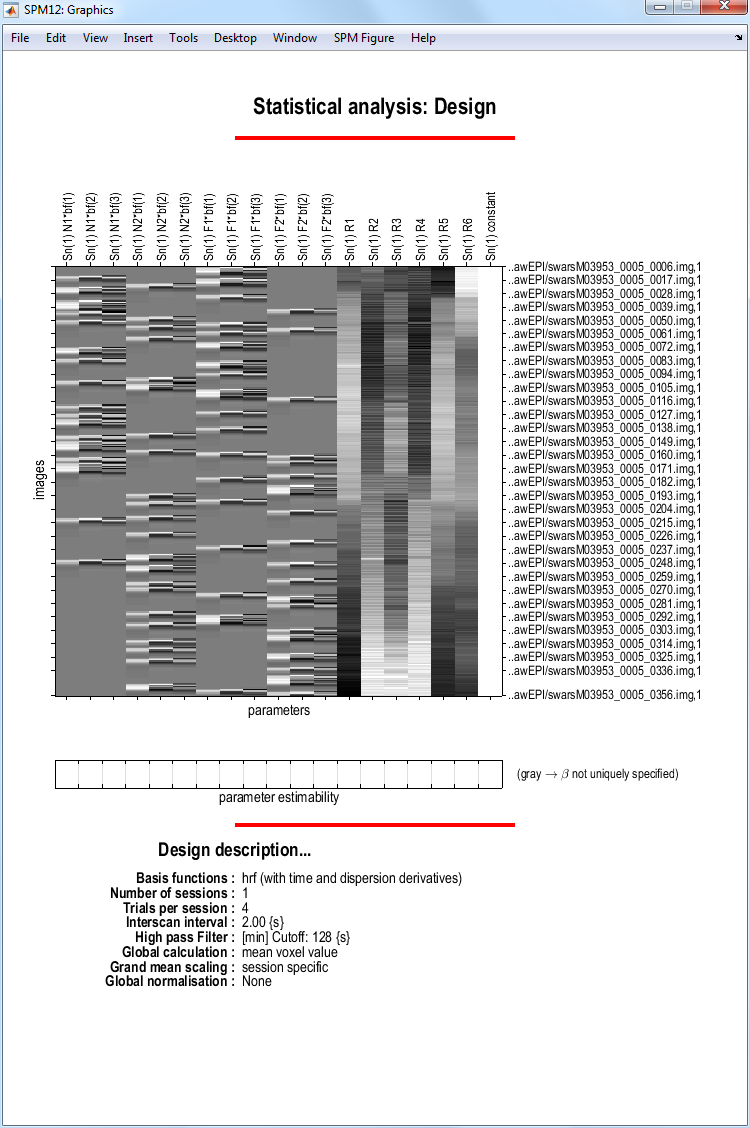
\includegraphics[width=100mm]{faces/cat_design}
\caption{\em \textbf{Design matrix}. \label{cat_design}}
\end{center}
\end{figure}

At this stage it is advisable to check your model specification using SPM's review facility which is accessed via the ``Review'' button. This brings up a ``design'' tab on the interactive window clicking on which produces a pulldown menu. If you select the first item ``Design Matrix'' SPM will produce the image shown in Figure~\ref{cat_design}. If you select ``Explore'' then ``Session 1'' then ``N1'', SPM will produce the plots shown in Figure~\ref{cat_explore}.
\begin{figure}
\begin{center}
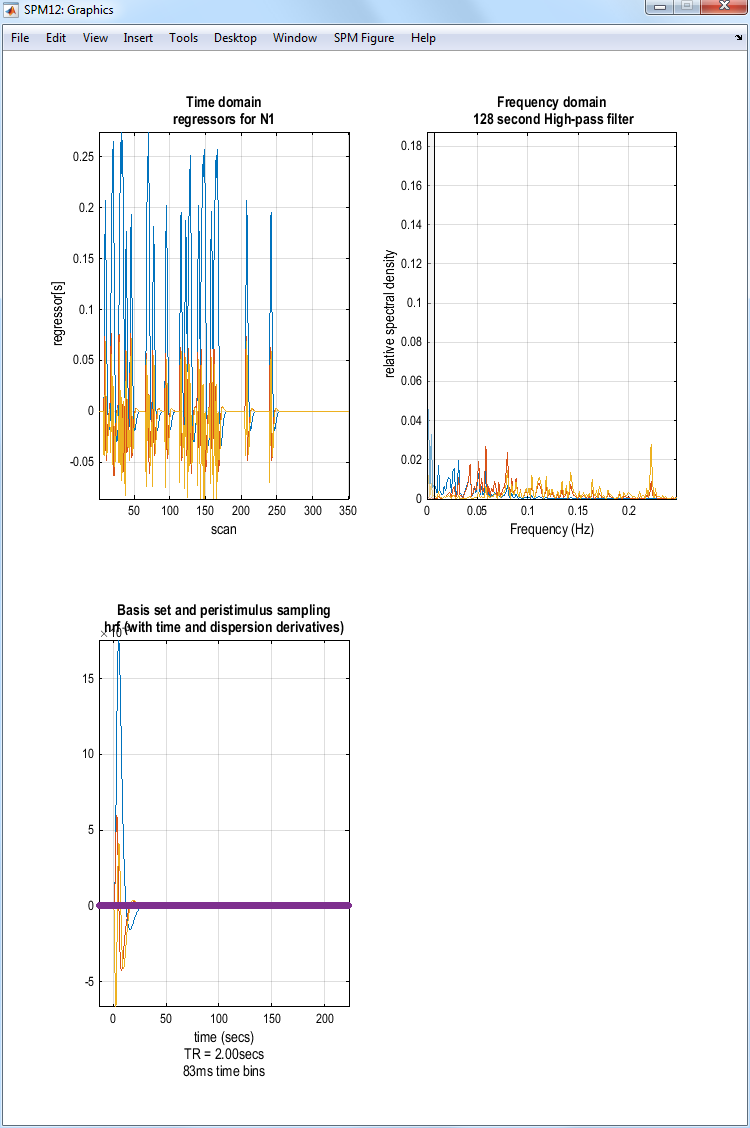
\includegraphics[width=100mm]{faces/cat_explore}
\caption{\em \textbf{Exploring the design matrix in Figure~\ref{cat_design}}. This shows the time series of the ``N1'' regressor (top left), the three basis functions used to convert assumed neuronal activity into hemodynamic activity (bottom left), and a frequency domain plot of the three regressors for the basis functions in this condition (top right). The frequency domain plot shows that the frequency content of the ``N1'' condition is generally above the set frequencies that are removed by the High Pass Filter (HPF) (these are shown in gray - in this model we accepted the default HPF cut-off of 128s or 0.008Hz). \label{cat_explore}}
\end{center}
\end{figure}

\subsection{Estimate}

Press the \textsc{Estimate} button. This will call up the specification of an fMRI estimation job in the batch editor window. Then
\begin{itemize}
\item Highlight the ``Select SPM.mat'' option and then choose the \texttt{SPM.mat} file saved in the \texttt{DIR/categorical} directory.
\item Save the job as \texttt{categorical\_est.job} and press \texttt{Run} button.
\end{itemize}
SPM will write a number of files into the selected directory including an \texttt{SPM.mat} file.

\subsection{Inference for categorical design}

Press ``Results'' and select the SPM.mat file from \texttt{DIR/categorical}. This will again invoke the contrast manager. Because we specified that our model was using a ``Factorial design'' a number of contrasts have been specified automatically, as shown in Figure~\ref{cat_contrasts}.
\begin{figure}
\begin{center}
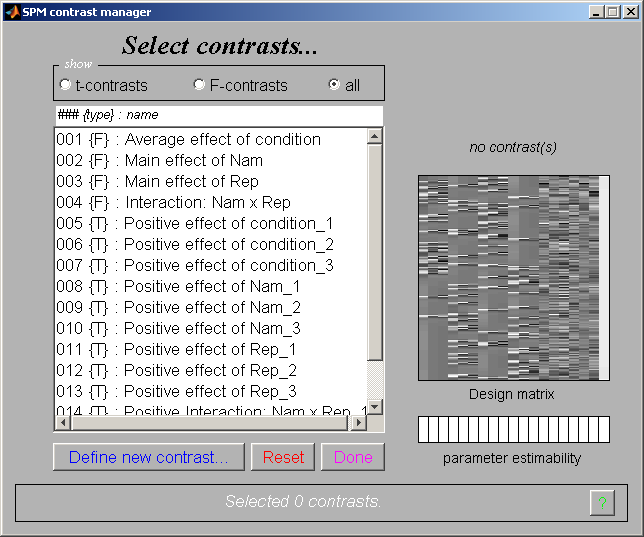
\includegraphics[width=100mm]{faces/cat_contrasts}
\caption{\em Contrast Manager containing default contrasts for categorical design. \label{cat_contrasts}}
\end{center}
\end{figure}

\begin{itemize}
\item Select contrast number 5. This is a t-contrast \texttt{Positive effect of condition\_1} This will show regions where the average effect of presenting faces is significantly positive, as modelled by the first regressor (hence the \texttt{\_1}), the canonical HRF. Press `Done''.
\item \emph{Mask with other contrast ? [Yes/No]}
\item Specify No.
\item \emph{Title for comparison ?}
\item Enter ``Canonical HRF: Faces $>$ Baseline''
\item \emph{p value adjustment to control: [FWE/FDR/none]}
\item Select FWE
\item \emph{Corrected p value(family-wise error)}
\item Accept the default value, 0.05
\item \emph{Extent threshold \{voxels\} [0]}
\item Accept the default value, 0.
\end{itemize}
SPM will then produce the MIP shown in Figure~\ref{cat5_volume}.

\subsection{Statistical tables}

To get a summary of local maxima, press the ``whole brain'' button in the p-values section of the interactive window. This will list all clusters above the chosen level of significance as well as separate ($>$8mm apart) maxima within a cluster, with details of significance thresholds and search volume underneath, as shown in Figure~\ref{cat5_volume}
\begin{figure}
\begin{center}
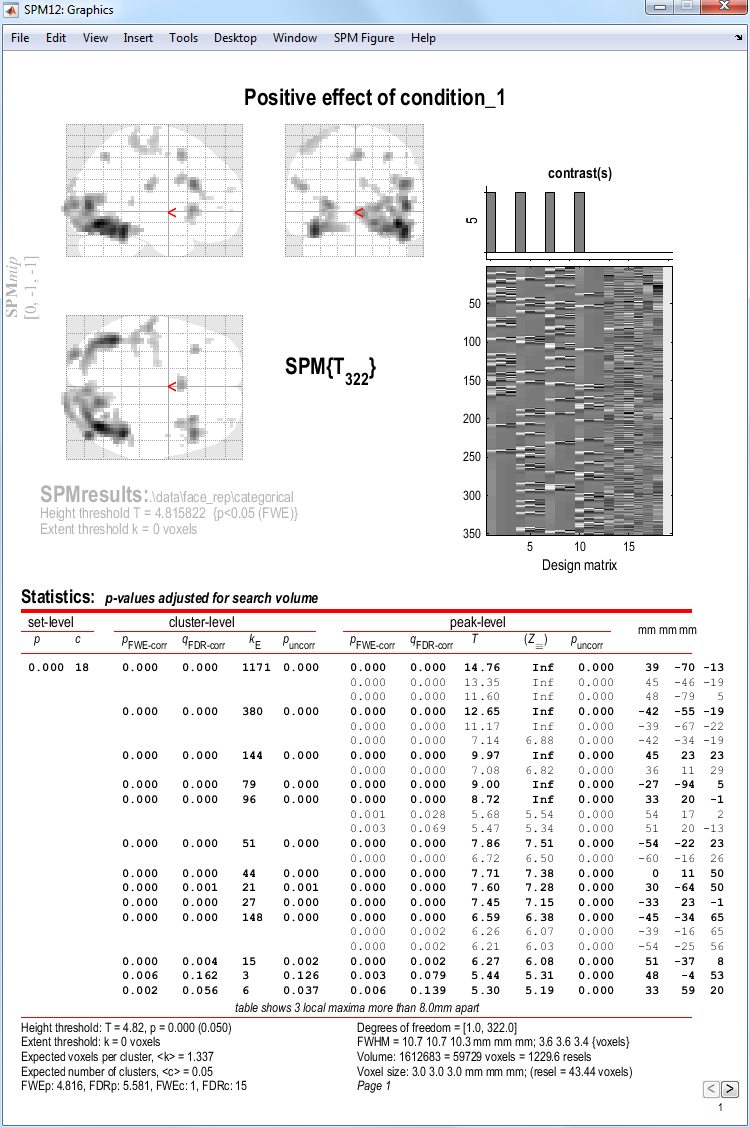
\includegraphics[width=100mm]{faces/cat5_volume}
\caption{\em \textbf{MIP and Volume table for Canonical HRF}: Faces  $>$ Baseline. \label{cat5_volume} }
\end{center}
\end{figure}

The columns in volume table show, from right to left:
\begin{itemize}
\item \textbf{x, y, z (mm)}: coordinates in MNI space for each maximum.
\item \textbf{peak-level}: the chance (p) of finding (under the null hypothesis) a peak with this or a greater height (T- or Z-statistic), corrected (FWE or FDR)/ uncorrected for search volume.
\item \textbf{cluster-level}: the chance (p) of finding a cluster with this many(ke) or a greater number of voxels, corrected (FWE or FDR)/ uncorrected for search volume.
\item \textbf{set-level}: the chance (p) of finding this (c) or a greater number of clusters in the search volume.
\end{itemize}

Right-click on the MIP and select ``goto global maximum''. The cursor will move to [39 -70 -14]. You can view this activation on the subject's normalised, attenuation-corrected structural (\texttt{wmsM03953\_0007\.img}), which gives best anatomical precision, or on the normalised mean functional (\texttt{wmeansM03953\_0005\_0006.img}), which is closer to the true data and spatial resolution (including distortions in the functional EPI data). 

If you select ``plot'' and choose ``Contrast of estimates and 90\% C.I'' (confidence interval), and select the ``Average effect of condition'' contrast, you will see three bars corresponding to the parameter estimates for each basis function (summed across the 4 conditions). The BOLD impulse response in this voxel loads mainly on the canonical HRF, but also significantly (given that the error bars do not overlap zero) on the temporal and dispersion derivatives (see next Chapter).

\subsection{F-contrasts}

To assess the main effect of repeating faces, as characterised by both the hrf \emph{and} its derivatives, an F-contrats is required. This is really asking whether repetition changes the \emph{shape} of the impulse response (e.g, it might affect its latency but not peak amplitude), at least the range of shapes defined by the three basis functions. Because we have told SPM that we have a factorial design, this required contrast will have been created automatically - it is number 3. 

\begin{itemize}
\item Press ``Results'' and select the \texttt{SPM.mat} file in the \texttt{DIR/categorical} directory.
\item Select the ``F-contrast'' toggle and the contrast number 3, as shown in Figure~\ref{cat3_contrast}. Press ``Done''.
\item \emph{Mask with other contrast ? [Yes/No]}.
\item Specify ``Yes''.
\item Select contrast 5 - \texttt{Positive effect of condition\_1} (the T-contrast of activation versus baseline, collapsed across conditions, that we evaluated above)
\item \emph{uncorrected mask p-value ?}
\item Change to 0.001
\item \emph{nature of mask?}
\item Select 'inclusive'
\item \emph{Title for comparison ?}
\item Keep ``Main effect of Rep (masked with ...)''
\item \emph{p value adjustment to control: [FWE/none]}
\item Select none
\item \emph{threshold (F or p value)}
\item Accept the default value, 0.001
\item \emph{Extent threshold \{voxels\} [0]}
\item Accept the default value, 0
\end{itemize}

A MIP should then appear, the top half of which should look like Figure~\ref{cat3_psth}.

\begin{figure}
\begin{center}
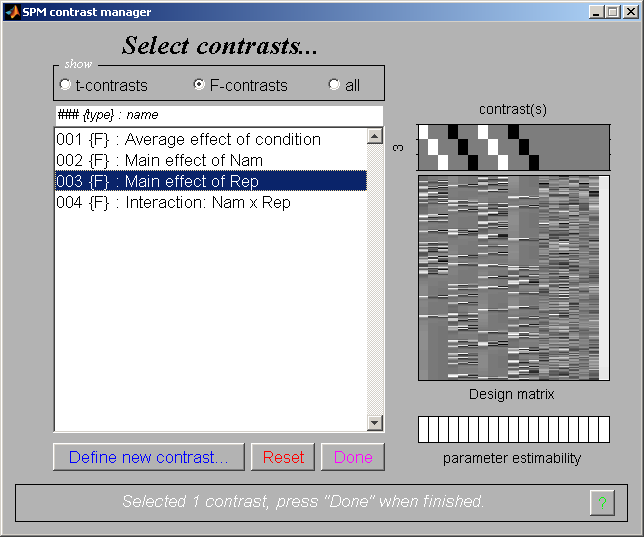
\includegraphics[width=100mm]{faces/cat3_contrast}
\caption{\em Contrast manager showing selection of the first contrast ``Main effect of Rep'' (repetition: F1 and N1 vs F2 and N2)\label{cat3_contrast} }
\end{center}
\end{figure}

\begin{figure}
\begin{center}
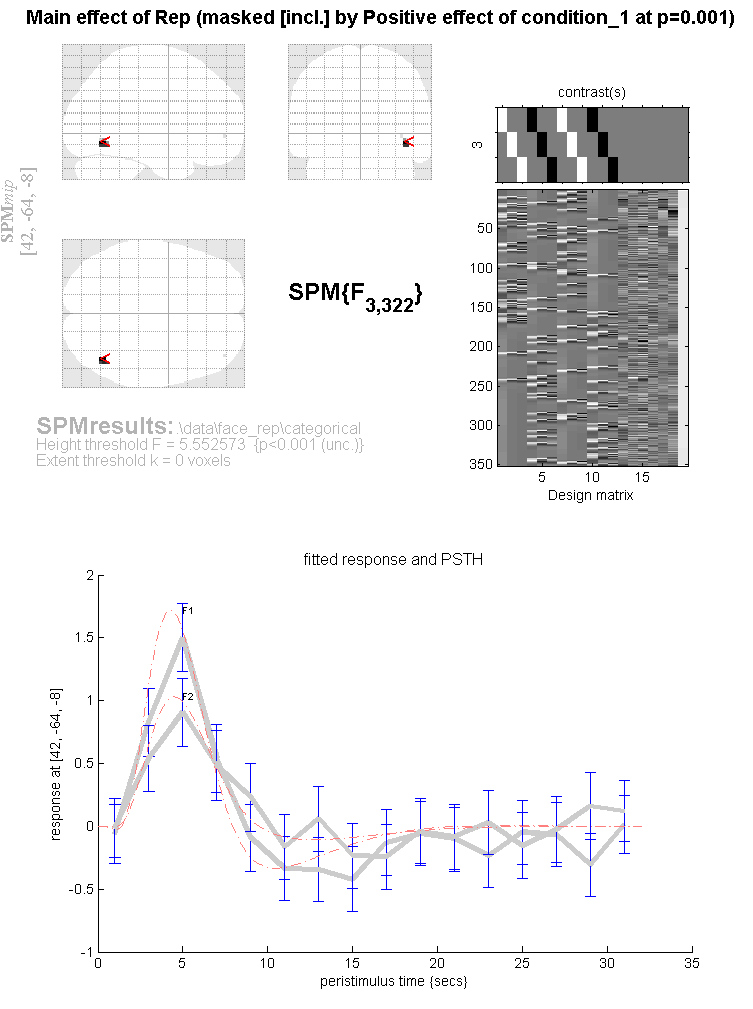
\includegraphics[width=100mm]{faces/cat3_psth}
\caption{\em MIP for Main effect of Rep, masked inclusively with Canonical HRF: Faces  $>$ Baseline at p$<$.001 uncorrected. Shown below are the best-fitting responses and peri-stimulus histograms (PSTH) for F1 and F2. \label{cat3_psth} } 
\end{center}
\end{figure}

Note that this contrast will identify regions showing any effect of repetition (e.g, decreased or increased amplitudes) \emph{within} those regions showing activations (on the canonical HRF) to faces versus baseline (at p$<$.05 uncorrected). Select ``goto global max'', which is in right ventral temporal cortex [42 -64 -8].

If you press plot and select ``Event-related responses'', then ``F1'', then ``fitted response and PSTH'', you will see the best fitting linear combination of the canonical HRF and its two derivatives (thin red line), plus the ``selectively-averaged'' data (peri-stimulus histogram, PSTH), based on an FIR refit (see next Chapter). 
If you then select the ``hold'' button on the Interactive window, and then ``plot'' and repeat the above process for the ``F2'' rather than ``F1'' condition, you will see two estimated event-related responses, in which repetition decreases the peak response (ie F2$<$F1), as shown in Figure~\ref{cat3_psth}.

You can explore further F-contrasts, which are a powerful tool once you understand them. For example, the MIP produced by the ``Average effect of condition'' F-contrast looks similar to the earlier T-contrast, but importantly shows the areas for which the sums across conditions of the parameter estimates for the canonical hrf \emph{and/or} its temporal derivative \emph{and/or} its dispersion derivative are different from zero (baseline). The first row of this F-contrast ([1 0 0 1 0 0 1 0 0 1 0 0]) is also a two-tailed version of the above T-contrast, ie testing for both activations and deactivations versus baseline. This also means that the F-contrasts [1 0 0 1 0 0 1 0 0 1 0 0] and [-1 0 0 -1 0 0 -1 0 0 -1 0 0] are equivalent. Finally, note that an F- (or t-) contrast such as [1 1 1 1 1 1 1 1 1 1 1], which tests whether the mean of the canonical hrf AND its derivatives for all conditions are different from (larger than) zero is not sensible. This is because the canonical hrf and its temporal derivative may cancel each other out while being significant in their own right. The basis functions are really quite different things, and need to represent separate rows in an F-contrast. 

\subsection{F-contrasts for testing effects of movement}

To assess movement-related activation
\begin{itemize}
\item Press ``Results'', select the \texttt{SPM.mat} file, select ``F-contrast'' in the Contrast Manager. Specify e.g. ``Movement-related effects'' (name) and 
in the ``contrasts weights matrix'' window, or ``1:12 19'' in the ``columns for reduced design'' window.
\item Submit and select the contrast, specify ``mask with other contrasts?'' (no), ``title for comparison'' (accept default), ``corrected height threshold'' (FWE), and ``corrected p-value'' (accept default). 
\item When the MIP appears, select ``sections'' from the ``overlays'' pulldown menu, and select the normalised structural image (\texttt{wmsM03953\_0007.img}).
\end{itemize}

You will see there is a lot of residual movement-related artifact in the data (despite spatial realignment), which tends to be concentrated near the boundaries of tissue types (eg the edge of the brain; see Figure~\ref{movements}). (Note how the MIP can be misleading in this respect, since though it appears that the whole brain is affected, this reflects the nature of the (X-ray like) projections onto each orthogonal view; displaying the same datae as sections in 3D shows that not every voxel is suprathreshold.)  Even though we are not interested in such artifact, by including the realignment parameters in our design matrix, we ``covary out'' (linear components) of subject movement, reducing the residual error, and hence improve our statistics for the effects of interest.

\begin{figure}
\begin{center}
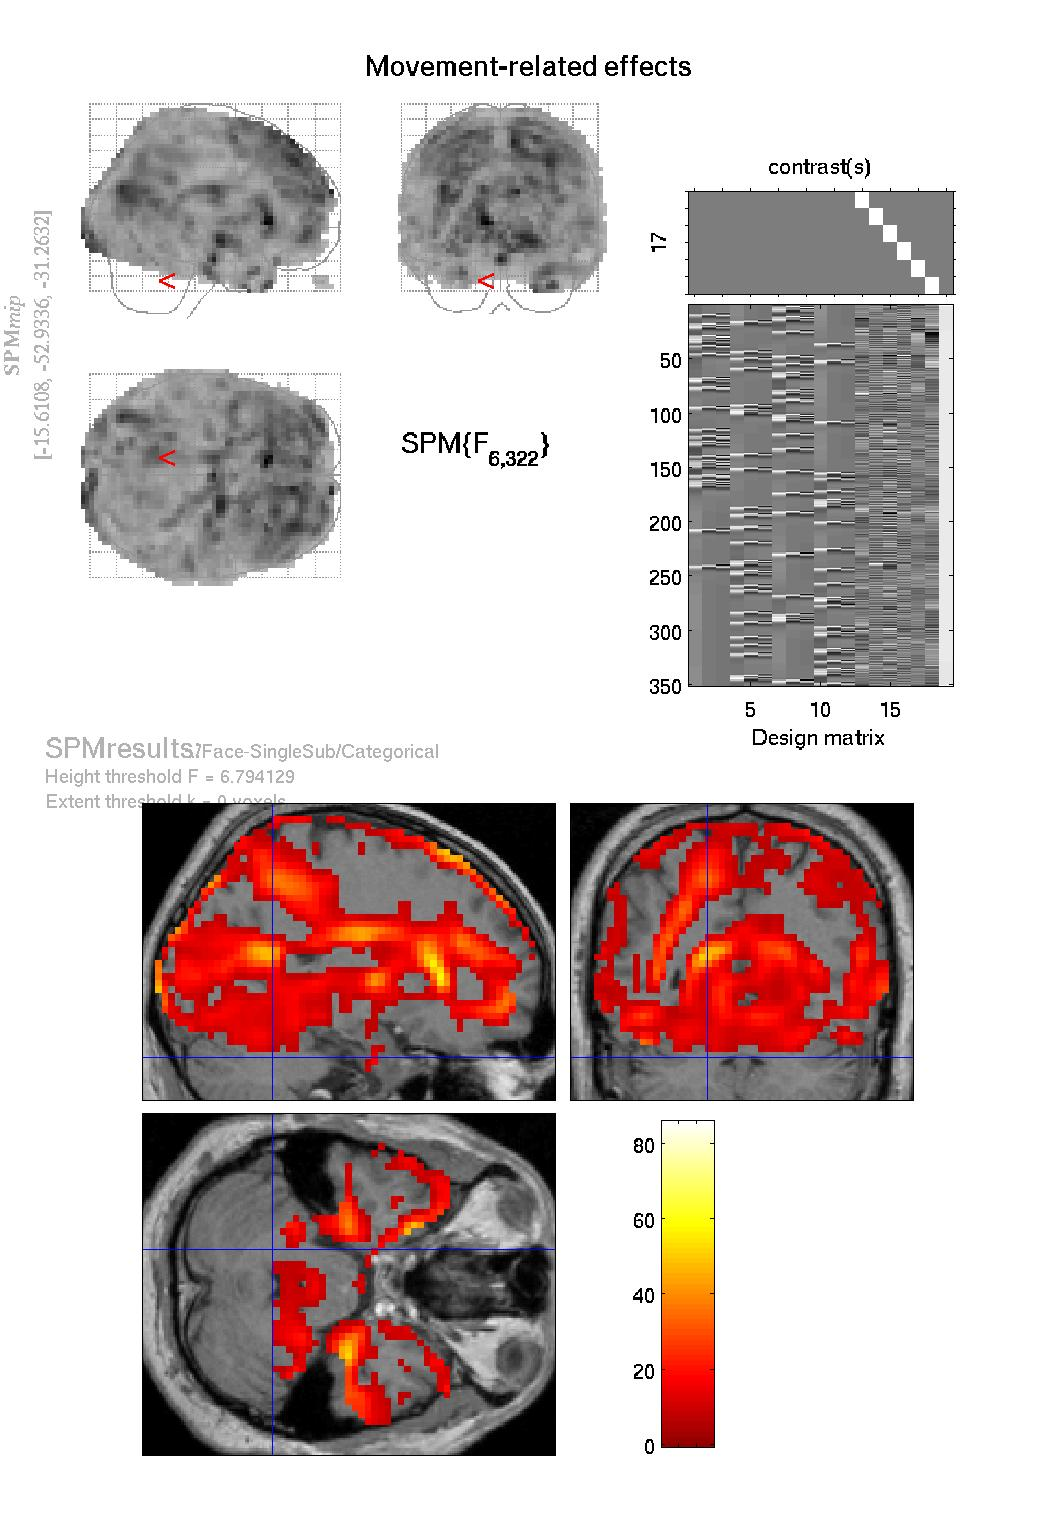
\includegraphics[width=100mm]{faces/movements}
\caption{\em Movement-related activations. These spurious `activations' are due to residual movement of the head during scanning. These effects occur at tissue boundaries and boundaries between brain and non-brain, as this is where contrast differences are greatest. Including these regressors in the design matrix means these effects cannot be falsely attributed 
to neuronal activity. \label{movements} }
\end{center}
\end{figure}

\section{Modelling parametric responses}

Before setting up the design matrix, we must first load into \matlab\ the Stimulus Onsets Times (SOTs), as before, and also the ``Lags'', which are specific to this experiment, and which will be used as parametric modulators. The Lags code, for each second presentation of a face (N2 and F2), the number of other faces intervening between this (repeated) presentation and its previous (first) presentation. Both SOTs and Lags are represented by Matlab cell arrays, stored in the \texttt{sots.mat} file.

\begin{itemize}
\item At the \matlab\ command prompt type \texttt{load sot}. This loads the stimulus onset times and the lags (the latter in a cell array called \texttt{itemlag}.
\end{itemize}

Now press the \textsc{Specify 1st-level} button. This will call up the specification of a fMRI specification job in the batch editor window. Then
\begin{itemize}
\item Press ``Load'' and select the \texttt{categorical\_spec.mat} job file you created earlier.
\item Open ``Conditions'' and then open the second ``Condition''.
\item Highlight ``Parametric Modulations'', select ``New Parameter''.
\item Highlight ``Name'' and enter ``Lag'', highlight values and enter \texttt{itemlag\{2\}}, highlight polynomial expansion and ``2nd order''.
\item Now open the fourth ``Condition'' under ``Conditions''.
\item Highlight ``Parametric Modulations'', select ``New Parameter''.
\item Highlight ``Name'' and enter ``Lag'', highlight values and enter \texttt{itemlag\{4\}}, highlight polynomial expansion and ``2nd order''.
\item Open ``Canonical HRF'' under ``Basis Functions'', highlight ``Model derivatives'' and select ``No derivatives'' (to make the design matrix a bit simpler for present purposes!).
\item Highlight ``Directory'' and select \texttt{DIR/parametric} (having ``unselected'' the current definition of directory from the Categorical analysis).
\item Save the job as \texttt{parametric\_spec} and press the \texttt{Run} button.
\end{itemize}

This should produce the design matrix shown in Figure~\ref{par_design}.

\begin{figure}
\begin{center}
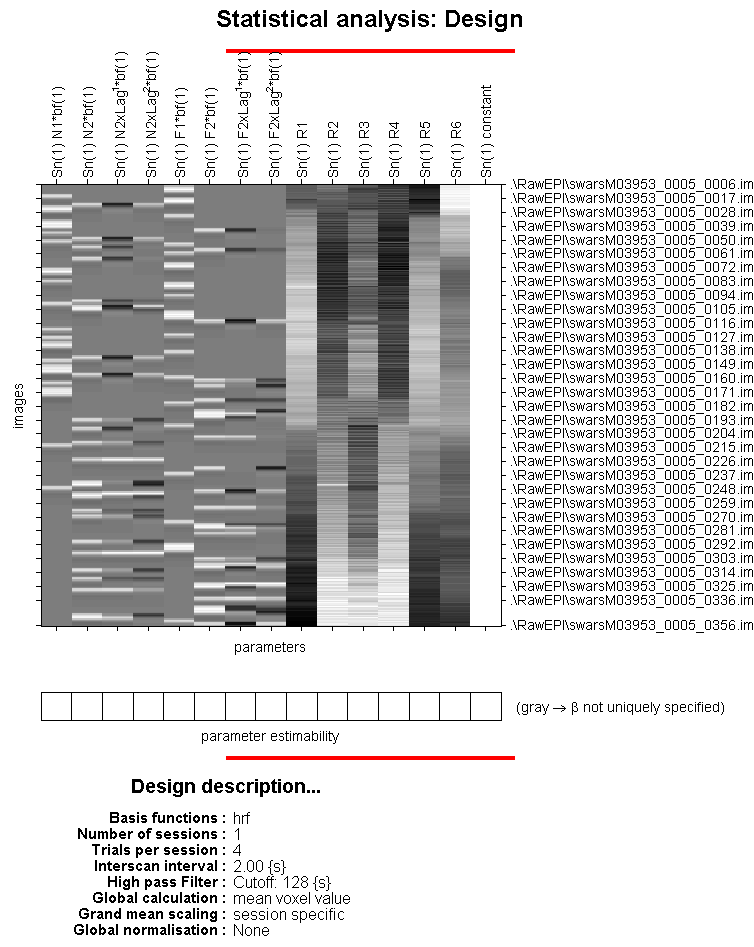
\includegraphics[width=100mm]{faces/par_design}
\caption{\em \textbf{Design matrix for testing repetition effects parametrically.} Regressor 2 indicates the second occurence of a nonfamous face. Regressor 3 modulates this linearly as a function of lag (ie. how many faces have been shown since that face was first presented), and regressor 4 modulates this quadratically as a function of lag. Regressors 6,7 and 8 play the same roles, but for famous faces. \label{par_design} }
\end{center}
\end{figure}

\subsection{Estimate}

Press the \textsc{Estimate} button. This will call up the specification of an fMRI estimation job in the batch editor window. Then
\begin{itemize}
\item Highlight the ``Select SPM.mat'' option and then choose the \texttt{SPM.mat} file saved in the \texttt{DIR/parametric} directory.
\item Save the job as \texttt{parametric\_est.job} and press the \texttt{Run} button.
\end{itemize}
SPM will write a number of files into the selected directory including an \texttt{SPM.mat} file.

\subsection{Plotting parametric responses}

We will look at the effect of lag (up to second order, ie using linear and quadratic terms) on the response to repeated Famous faces, within those regions generally activated by faces versus baseline. To do this
\begin{itemize}
\item Press ``Results'' and select the \texttt{SPM.mat} file in the \texttt{DIR/parametric} directory.
\item Press ``Define new contrast'', enter the name ``Famous Lag'', press the ``F-contrast'' radio button, enter ``1:6 9:15'' in the ``columns in reduced design'' window, press ``submit'', ``OK'' and ``Done''.
\item Select the ``Famous Lag'' contrast.
\item \emph{Mask with other contrast ? [Yes/No]}
\item Specify ``Yes''.
\item Select the ``Positive Effect of Condition 1'' T contrast.
\item Change to an 0.05 uncorrected mask p-value.
\item Nature of Mask ? inclusive.
\item \emph{ Title for comparison ?}
\item Accept what is offered
\item \emph{p value adjustment to control: [FWE/none]}
\item Select None
\item \emph{Threshold \{F or p value\}}
\item Accept the default value, 0.001
\item \emph{Extent threshold \{voxels\} [0]}
\item Accept the default value, 0.
\end{itemize}

Figure~\ref{famous_lag_mip} shows the MIP and an overlay of this parametric effect using overlays, sections and selecting the \texttt{wmsM03953\_0007.img} image. 
\begin{figure}
\begin{center}
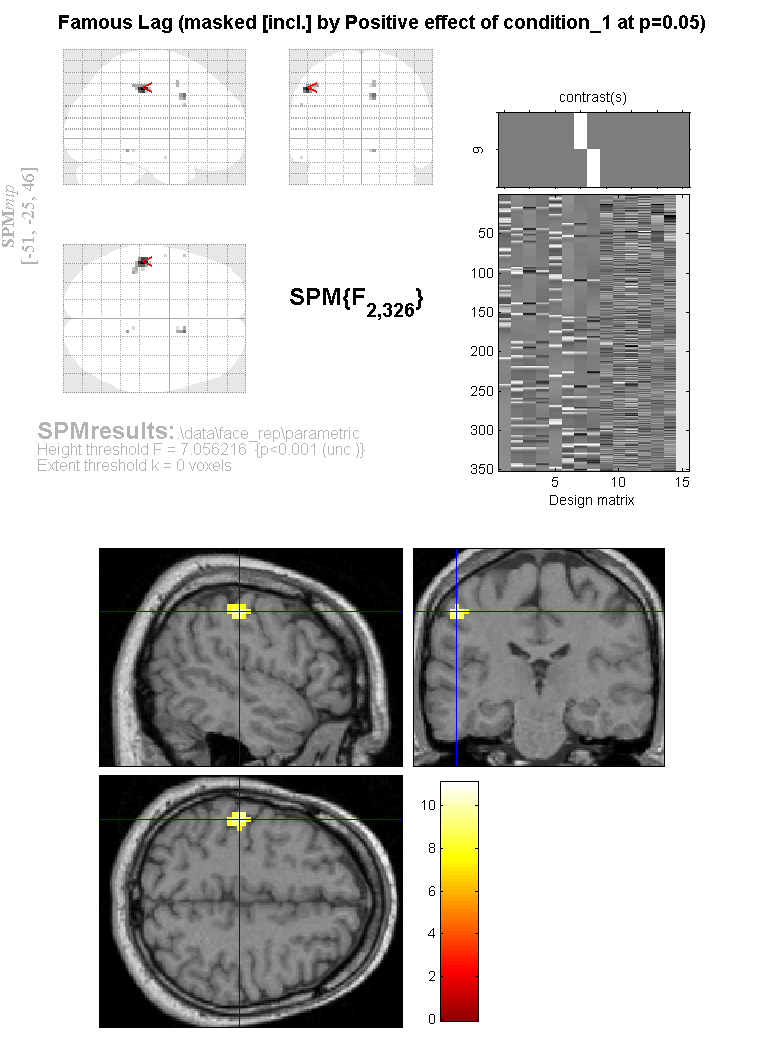
\includegraphics[width=100mm]{faces/famous_lag_mip}
\caption{\em MIP and overlay of parametric lag effect in parietal cortex. \label{famous_lag_mip} }
\end{center}
\end{figure}
The effect is plotted in the time domain in figure~\ref{famous_lag}. This was obtained by
\begin{itemize}
\item Right clicking on the MIP and selecting ``global maxima''.
\item Pressing Plot, and selecting ``parametric responses'' from the pull-down menu.
\item Which effect ? select ``F2''.
\end{itemize}

This shows a quadratic effect of lag, in which the response appears negative for short-lags, but positive and maximal for lags of about 40 intervening faces (note that this is a very approximate fit, since there are not many trials, and is also confounded by time during the session, since longer lags necessarily occur later (for further discussion of this issue, see the SPM2 example analysis of these data on the webpage).

\begin{figure}
\begin{center}
\includegraphics[width=150mm]{faces/famous_lag}
\caption{\em Response as a function of lag. \label{famous_lag} }
\end{center}
\end{figure}


\section{Bayesian analysis}

\subsection{Specification}

Press the \textsc{Specify 1st-level} button. This will call up an fMRI specification job in the batch editor window. Then

\begin{itemize}
\item Load the \texttt{categorical\_spec.mat} job file created for the classical analysis.
\item Open ``Subject/Session'', highlight ``Scans''.
\item Deselect the smoothed functional images using the `unselect all' option available from a right mouse click in the SPM file selector (bottom window).
\item Select the unsmoothed functional images using the \texttt{\textasciicircum wa.*} filter and ``select all'' option available from a right mouse click in the SPM file selector (top right window). The Bayesian analysis uses a spatial prior where the spatial regularity in the signal is estimated from the data. It is therefore not necessary to create smoothed images if you are only going to do a Bayesian analysis.
\item Press ``Done''.
\item Highlight ``Directory'' and select the \texttt{DIR/bayesian} directory you created earlier (you will first need to deselect the \texttt{DIR/categorical} directory).
\item Save the job as \texttt{specify\_bayesian.mat} and press the \texttt{Run} button.
\end{itemize}

\subsection{Estimation}

Press the \textsc{Estimate} button. This will call up the specification of an fMRI estimation job in the batch editor window. Then
\begin{itemize}
\item Highlight the ``Select SPM.mat'' option and then choose the \texttt{SPM.mat} file saved in the \texttt{DIR/bayesian} subdirectory
\item Highlight ``Method'' and select the ``Choose Bayesian 1st-level'' option.
\item Save the job as \texttt{estimate\_bayesian.job} and press the \texttt{Run} button.
\end{itemize}

\begin{figure}
\begin{center}
\includegraphics[width=100mm]{faces/face_ar1}
\caption{\em Bayesian analysis: Estimated AR(1) coefficient image indicating heterogeneity near the circle of Willis \label{face_ar1} }
\end{center}
\end{figure}

SPM will write a number of files into the output directory including 
\begin{itemize}
\item An \texttt{SPM.mat} file.
\item Images \texttt{Cbeta\_k.img} where $k$ indexes the $k$th estimated regression coefficient. These filenames are prefixed with a ``\texttt{C}''' indicating that these are the mean values of the ``Conditional'' or ``Posterior'' density.
\item Images of error bars/standard deviations on the regression coefficients \texttt{SDbeta\_k.img}.
\item An image of the standard deviation of the error \texttt{Sess1\_SDerror.img}.
\item An image \texttt{mask.img} indicating which voxels  were included in the analysis.
\item Images \texttt{Sess1\_AR\_p.img} where $p$ indexes the $p$th AR coefficient. See eg. Figure~\ref{face_ar1}.
\item Images \texttt{con\_i.img} and \texttt{con\_sd\_i.img} which are the mean and standard deviation of the $i$th pre-defined contrast.
\end{itemize}

\subsection{Inference}

After estimation, we can make a posterior inference using a PPM. Basically, we identify regions in which we have a high probability (level of confidence) that the response exceeds a particular size (eg, \% signal change). This is quite different from the classical inferences above, where we look for low probabilities of the null hypothesis that the size of the response is zero.

To determine a particular response size (``size threshold'') in units of PEAK \% signal change, we first need to do a bit of calculation concerning the scaling of the parameter estimates. The parameter estimates themselves have arbitrary scaling, since they depend on the scaling of the regressors. The scaling of the regressors in the present examples depends on the scaling of the basis functions. To determine this scaling, load the ``SPM.mat'' file and type in \matlab\ \texttt{sf = max(SPM.xBF.bf(:,1))/SPM.xBF.dt} (alternatively, press ``Design:Explore:Session 1'' and select any of the conditions, then read off the peak height of the canonical HRF basis function (bottom left)).

Then, if you want a size threshold of 1\% peak signal change, the value you need to enter for the PPM threshold (ie the number in the units of the parameter estimates) is \texttt{1/sf} (which should be 4.75 in the present case).\footnote{Strictly speaking, this is the peak height of the canonical component of the best fitting BOLD impulse response: the peak of the complete fit would need to take into account all three basis functions and their parameter estimates.}

Finally, if we want to ask where is there a signal greater than 1\% (with a certain confidence) to faces versus baseline, we need to create a new contrast that takes the AVERAGE of the parameter estimates for the canonical HRF across the four conditions (N1 to F2), rather than the default \texttt{Positive effect of condition\_1} contrast, which actually calculates the SUM of the parameter estimates for the canonical HRF across conditions (the average vs sum makes no difference for the classical statistics).

\begin{itemize}
\item Press ``Results''.
\item Select the \texttt{SPM.mat} file created in the last section.
\item Press ``Define new contrast'', enter the name ``AVERAGE Canonical HRF: Faces $>$ Baseline'', press the ``T-contrast'' radio button, enter the contrast [1 0 0 1 0 0 1 0 0 1 0 0]/4, press ``submit'', ``OK'' and ``Done''.
\item \emph{Mask with other contrast ? [Yes/No]}
\item Specify No
\item \emph{Title for comparison}
\item Enter ``AVERAGE Canonical HRF: Faces $>$ Baseline''
\item \emph{Effect size threshold for PPM}
\item Enter the value
\item \emph{Posterior probability threshold for PPM}
\item Enter the value 0.95
\item \emph{Extent threshold [0]}
\item Accept the default value
\item \emph{Plot effect size [Yes/No]}
\item Select the default ``Yes''
\end{itemize}
SPM will then plot a map of effect sizes at voxels where it is 95\% sure that the effect size is greater than 1\% of the global mean.
Then use overlays, sections, select the normalised structural image created earlier and move the cursor to the activation in the left hemisphere. This should create the plot shown in Figure~\ref{face_bayes}.

\begin{figure}
\begin{center}
\includegraphics[width=100mm]{faces/face_bayes}
\caption{\em Bayesian analysis: MIP and overlay of effect sizes at voxels where PPM is 95\% sure that the effect size is greater than 1\% of the global mean. The cursor is at the location $x=30,y=-82,z=-17$mm\label{face_bayes} }
\end{center}
\end{figure}


\bibliography{methods_macros,methods_group,external}

\parskip=0mm

\end{document}

